\documentclass[11pt]{beamer}
\usepackage[utf8]{inputenc}
\usepackage[T1]{fontenc}
\usepackage{lmodern}
\usepackage{amsmath}
\usepackage{hyperref}
\usepackage{array}
\usepackage{amsfonts}
\usepackage{amssymb}
\usepackage{graphicx}
\usepackage{epstopdf}
\usepackage{caption}
\usepackage{multicol}
\usepackage{listings}
\usepackage{alltt}
\usepackage[makeroom]{cancel}
\usetheme{Frankfurt}
\usepackage{tikz}
\usetikzlibrary{patterns}
\usetikzlibrary{plotmarks}
\titlegraphic{\vspace{8cm}}% to push the other text to the top
\addtobeamertemplate{navigation symbols}{}{%
	\usebeamerfont{footline}%
	\usebeamercolor[fg]{footline}%
	\hspace{1em}%
	\insertframenumber/\inserttotalframenumber
	\setbeamercolor{footline}{fg=blue}
	\setbeamerfont{footline}{series=\bfseries}
}
\newcolumntype{M}[1]{>{\centering\arraybackslash}m{#1}}
\begin{document}
	\author{
		Departamento de Investigacion en F\'isica \\
		Maestr\'ia en Ciencias (F\'isica)\\
		Hiram Ernesto Dami\'an}
	\title{Search for production of a Higgs boson and a single top quark in $\mu\mu$ final states in proton collisions at $\sqrt{s}=13$ TeV}
	%\subtitle{}
	\logo{
\includegraphics[scale=0.1]{unison-logo.png}}
	\institute{Universidad de Sonora}
	%\date{}
	%\subject{}
	\newcommand{\subf}[2]{%
		{\small\begin{tabular}[t]{@{}c@{}}
				#1\\#2
		\end{tabular}}%
	}
	%\setbeamercovered{transparent}
	%\setbeamertemplate{navigation symbols}{}
	\begin{frame}
	\titlepage
\end{frame}

\begin{frame}
\tableofcontents
\frametitle{Contenido}
\end{frame}


\begin{frame}
\section{Overview and motivation}
\frametitle{Overview}
\begin{itemize}
\item Through this project we will investigate the production of Higgs boson in association with a
single top quark (tH) in proton-proton collisions with the CMS experiment of the LHC. This
mechanism of production of the Higgs boson has not been observed before by any
experiment.

\item Understanding the production of the Higgs boson, as well as its decays are an important part
of the physical program of the CERN international laboratory experiments that try to complete
the tests to verify the Standard Model, the theory of the fundamental particles

\end{itemize}
\end{frame}


\begin{frame}
\frametitle{Motivation  for single top Higgs (tH)}
\begin{itemize}
\item Coupling measurement is essential to establish the nature of the Higgs
\item The exploration of Higgs production on the tH channel is subject relatively new. Measurements of CMS and ATLAS are compatible with SM predictions.
\item The tH study explores the relative sign of top-Higgs  and W-Higgs couplings.\\ Small deviations from SM predictions could be associated with physics beyond the
standard model (BSM) such as String Theory and  Supersymmetry.
\end{itemize}
\end{frame}

\begin{frame}
\section{Higgs theory}
\frametitle{Standard Model}
\begin{center}
\begin{figure}
	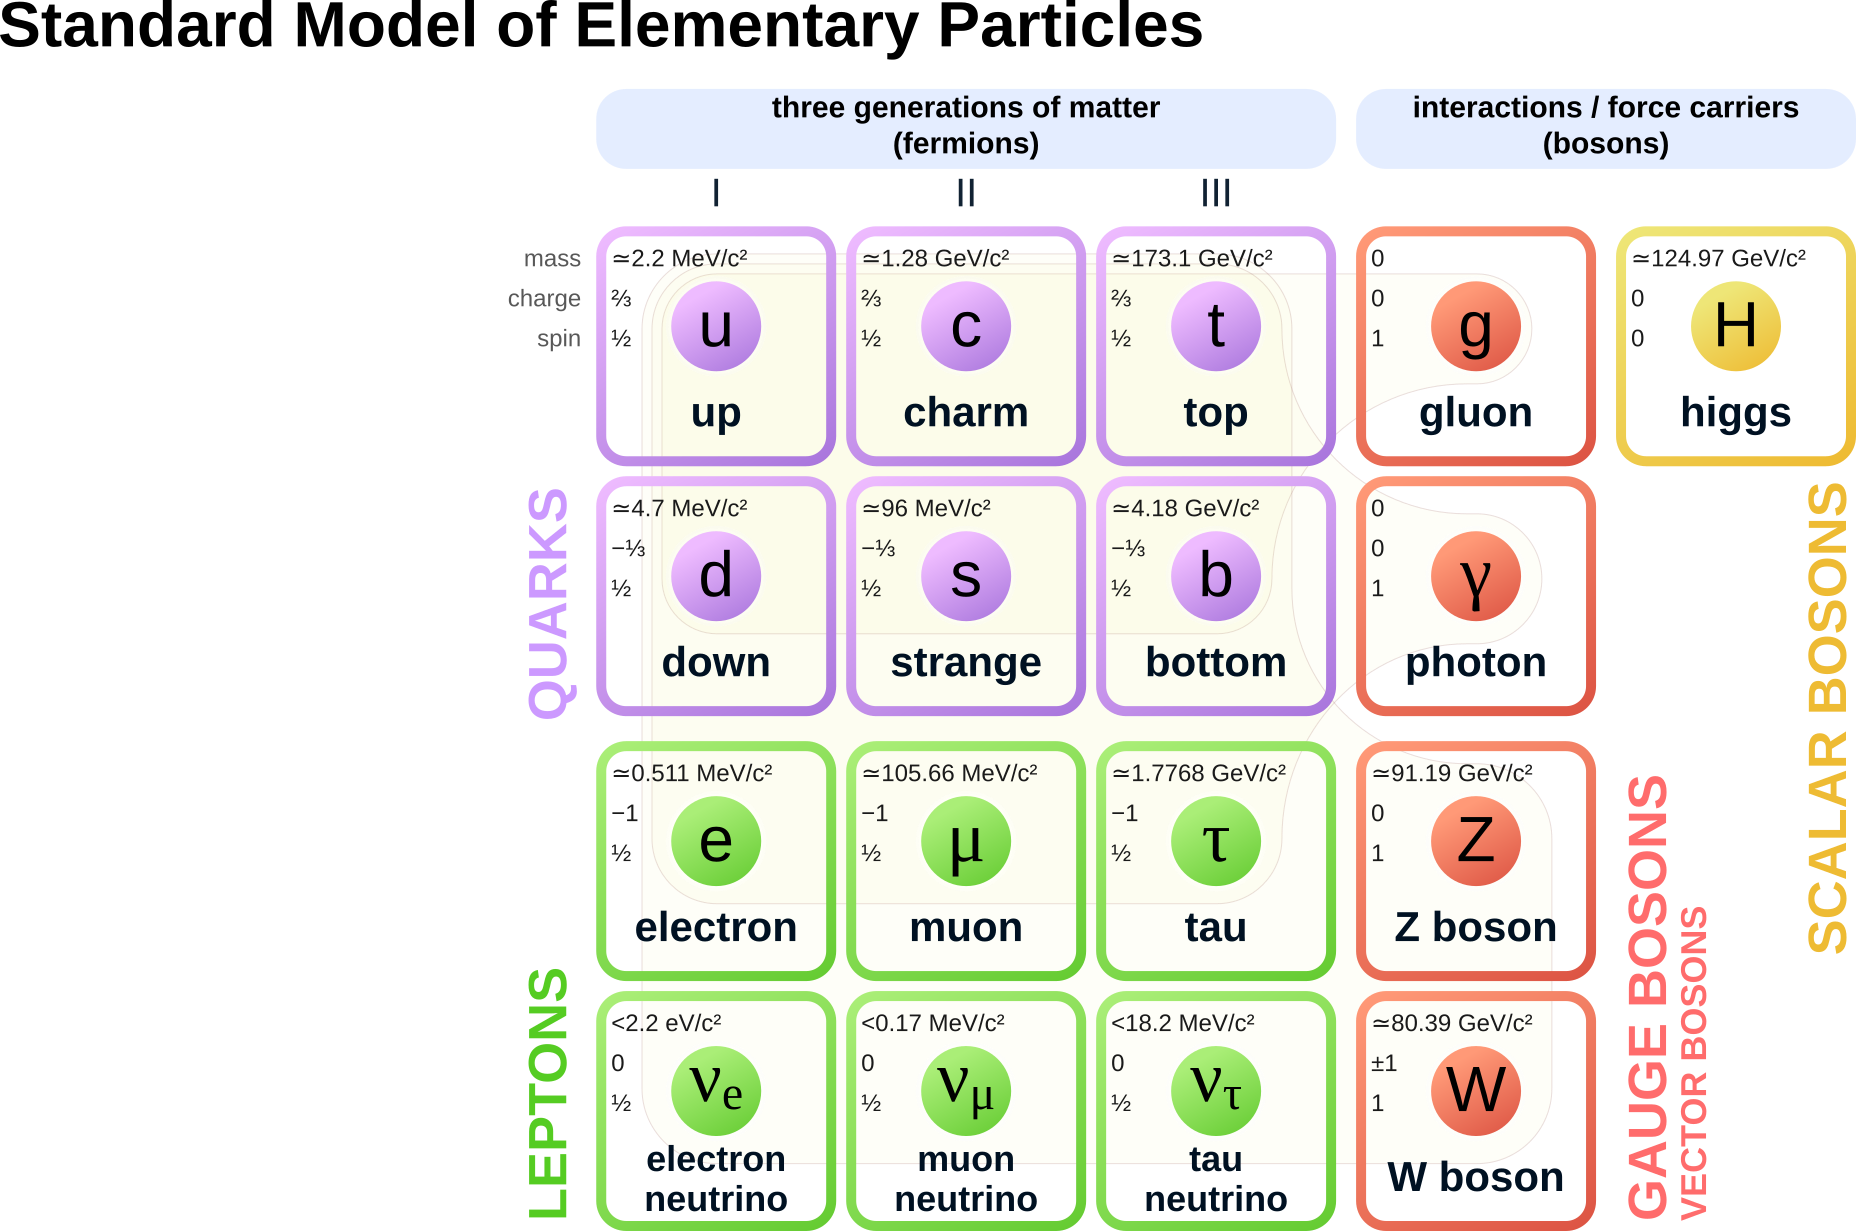
\includegraphics[width=9cm,height=6.5cm]{figures/sm1.png}
\end{figure}
\end{center}
\end{frame}

\begin{frame}
\frametitle{Electroweak SM Lagrangian}
The standard model is a theory of fields with spins 0, $\frac{1}{2}$ and 1. 
The  SM lagrangian 	
\begin{align*}
\mathcal{L}=\mathcal{L}_\text{gauge}+\mathcal{L}_f +\mathcal{L}_\text{higgs} + \mathcal{L}_\text{yukawa}
\end{align*}
donde 
\begin{itemize}
	\item $\mathcal{L}_\text{gauge}$=$ -\frac{1}{4}\left[F^{\mu\nu}F_{\mu\nu}\right]-\frac{1}{4}\left[G^{i\mu\nu}G^i_{\mu\nu}\right]$ 
	\begin{itemize}
		\item  $F^{\mu \nu}=\partial_\mu B_\nu -\partial_\nu B_\mu $
		\item  $G^{i\mu\nu}=\partial_\mu W^i_\nu -\partial_\nu W^i_\mu -g\epsilon^{ijk}W^j_\mu W^k_\nu $
	\end{itemize}
	\item $\mathcal{L}_f=i\bar{\Psi}_L \cancel{D}{\Psi}_L+i\bar{\psi}_R \cancel{D}{\psi}_R  $ is the kinematic term for fermions 
	\begin{itemize}
		\item $D_\mu {\Psi}_L=\left(\partial_\mu+igW_\mu+ig'Y_LB_\mu\right)\Psi_L$
		\item $D_\mu \psi_R=\left(\partial_mu +ig' Y_RB_\mu\right)\psi_R $
		\item g and g are boson coupling constants.
\footnote{L(R) refers to Left and right fields.
Y is the  weak hypercharge,Y=T$^3$-Q.Q is charge of particle field and T is weak isospin. $T^3=\pm 1/2$ for left handed doublets and $T^3=0$ for right handed singlets.}  
	\end{itemize}
\end{itemize}
%\begin{equation}
%\begin{split}
%\mathcal{L}=-\frac{1}{2}\text{Tr}\left[F^{\mu\nu}F_{\mu\nu} \right]+\bar{\Psi_L}i\gamma^\mu D_\mu \Psi_L  
%+\text{Tr}\left[(D_\mu \Phi)^\dagger (D^\mu \Phi)\right]+\mu^2 \Phi^\dagger \Phi  \\
%-\frac{1}{2}  \lambda (\Phi^\dagger \Phi)^2 & +\left(\frac{1}{2}\Psi_L^T Ch \Phi \Psi_L +h.c \right)
%\end{split}
%\end{equation}
%The matrix C in the last term is the charge conjugation matrix acting on the spinors, h is a matrix of Yukawa couplings
\end{frame}

\begin{frame}
\frametitle{Electroweak SM Lagrangian}
Higgs lagrangian 
\begin{align}
\mathcal{L}_{\text{Higgs}}=(D_\mu \Phi)^\dagger (D^\mu \Phi)-V(\Phi^\dagger \Phi)
\end{align}

with
\begin{itemize}
	\item $D_\mu \Phi = \left(\partial_\mu+(ig/2)\sigma^iW^i_\mu-i\frac{1}{2} g' B_\mu \right) \Phi $
	\item $V(\Phi^\dagger \Phi)=-\mu^2 \Phi^\dagger \Phi +\frac{1}{2}  \lambda (\Phi^\dagger \Phi)^2, \quad \mu^2>0  $ 
	\item $\Phi=\left(\begin{array}{c}
	\phi^+ \\
	\phi^0
	\end{array} \right)  $ is a SU(2) doublet.
	\item $\sigma^i$ are the Pauli matrices.
\end{itemize}
 
\begin{itemize}
	\item $\Phi$ is higgs field which is a complex scalar field. $\Phi$
	%\item  W$_\mu$ and B$_\mu$ are gauge bosons
	%\item g and g are boson coupling constants.
	\item $\lambda $ and $\mu^2$ are Higgs potential parameters
\end{itemize}
\end{frame}

\begin{frame}
\frametitle{SM Lagrangian}
Yukawa lagrangian
\begin{align}
\mathcal{L}_{yukawa}=\Gamma^u_{mn}q_{m\text{,}L} \tilde{\phi} u_{n\text{,}R}+\Gamma^d_{mn}\bar{q}_{m\text{,}L} \phi d_{n\text{,}R}+\Gamma^e_{mn}\bar{l}_{m\text{,}L} \phi e_{n\text{,}R}+h.c
\end{align}
\scriptsize{where h.c is hermitian conjugate.\\
The matrices $\Gamma_{mn}$ describe the so called Yukawa couplings between higgs doublet $\phi$ and the fermions.\\
Choosing}
\begin{align*}
\Phi=-\frac{1}{2}\left(\begin{array}{c}
0 \\
v+h
\end{array} \right) \rightarrow  \Phi=\frac{1}{2}\left(\begin{array}{c}
0 \\
v
\end{array} \right)
\end{align*}
\scriptsize{
By using it on the first part of 
the lagrangian it is obtained } 
\begin{align*}
	\frac{f_u v}{\sqrt{2}(\bar{u_L}u_R+\bar{u_R}u_L)}
\end{align*}
\scriptsize{
from which the masses for the fermions in question can be read off:}
\begin{align*}
m_=-\frac{f_uv}{\sqrt{2}}
\end{align*}
which m is the mass of fermions 
\end{frame}

\begin{frame}
\section{tH mechanisms}
\frametitle{Higgs production mechanisms}
\begin{center}
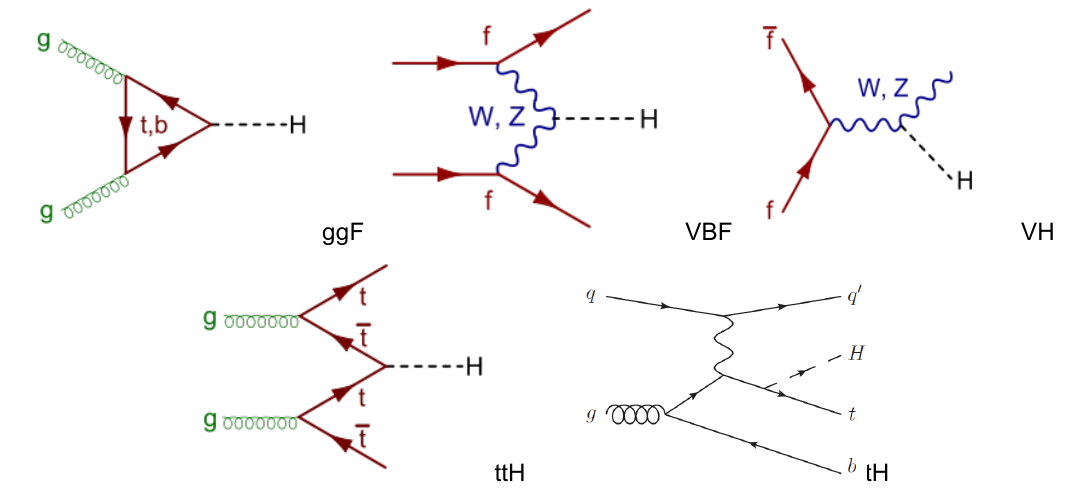
\includegraphics[scale=0.4]{figures/pg.png}
\end{center}
\end{frame}

\begin{frame}
\frametitle{tH production mechanisms}
\begin{center}
\begin{figure} 
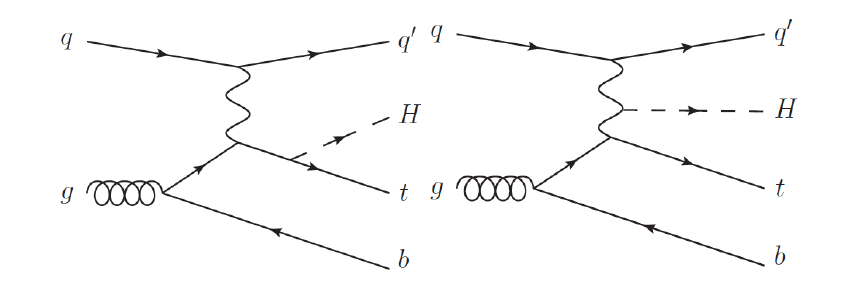
\includegraphics[scale=0.4]{figures/tq.png} 
\caption{tH mechanism. Higgs radiated from a top quark (left). Higgs radiated from a W boson (right)} 
\label{th}
\end{figure}
\end{center}
\end{frame}

\begin{frame}
\frametitle{tH production mechanisms}
\begin{itemize}
\item In a proton proton collision, the production cross section of the single top plus Higgs boson (tHq) process is driven by a
destructive interference of two main diagrams (see Fig. \ref{th}.), where the Higgs couples to either
the W boson or the top quark. 
\item  A second process, where the Higgs and top quark
are accompanied by a W boson (tHW) has similar behavior, albeit with a weaker interference
pattern.
\item However, in the presence of new physics, there may be relative opposite signs between the tH
and WH couplings which lead to constructive interference and enhance the cross sections by
an order of magnitude or more.
\end{itemize}
\end{frame}


\begin{frame}
\section{Production cross section}
\frametitle{Cross section}
\begin{itemize}
\item Classical definition: When two particles interact, cross section is the area transverse to their relative motion within
which they must meet in order to scatter from each other.
\item Quantum definition: Cross section describes the likelihood of two particles interacting under certain conditions\cite{1}
\item Experimentally
\begin{align}
d\sigma=\frac{\text{number of particles scattered into solid angle} \Delta\Omega}{\text{(number of particles incident)(scattering centers/area)}}
\end{align}
\item Cross sections are expressed in barns , where 1 barn=$10^{-34}$ cm$^{-2}$ 
\end{itemize}
\end{frame}

\begin{frame}
\frametitle{Cross section}
\begin{center}
	\begin{figure}
		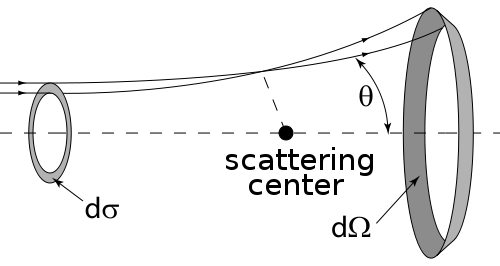
\includegraphics[scale=0.5]{figures/cs1.png}
		\caption{Drawing of an idealized scattering process showing the differential solid angle $\Delta\Omega$ and the
			scattering angle $\theta$}
	\end{figure}
\end{center}
\end{frame}

\begin{frame}
\frametitle{Cross section}
The reaction rate $N_R$ is determined by the total cross section $\sigma$ and the incident flux L.\\
L is called luminosity and it is measured in cm$^{-1}$s$^{-1}$. 
\begin{align}
N_R=\sigma \text{L}
\end{align}
\end{frame}



\begin{frame}
\frametitle{Higgs production Cross section}
\begin{table}
	\caption*{Higgs boson production cross sections  in pp collisions for $\sqrt{s}=13$TeV  (in
		pico barn).Integrated luminosity of 35.9 fb$^{-1}$ for Run 2\footnotemark}
	\begin{tabular}{|c|c|c|}
		\hline
		Production mechanism &
		$\sigma$ (picobarns pb)
		&Number of events \\
		\hline
		ggF &
		48.93 &
		1756587\\
		\hline
		VBF &
		3.78&
		135702\\
		\hline
		WH & 1.35 & 48465\\
		\hline
		ZH &0.88 & 31592\\
		\hline
		t$\bar{t}$H &
		0.50&
		18255\\
		\hline
		tH	(only)&
		0.015&
		560.39\\
		\hline
	\end{tabular}
\end{table}

\footnotetext[1]{\tiny{Data taken from The cern collaborarion “Higgs Physics the HL-LHC and HE-LHC” 2019, CERN-LPCC-2018-04}}

\end{frame}

\begin{frame}
\frametitle{Higgs production cross section}
\begin{center}
\begin{figure}
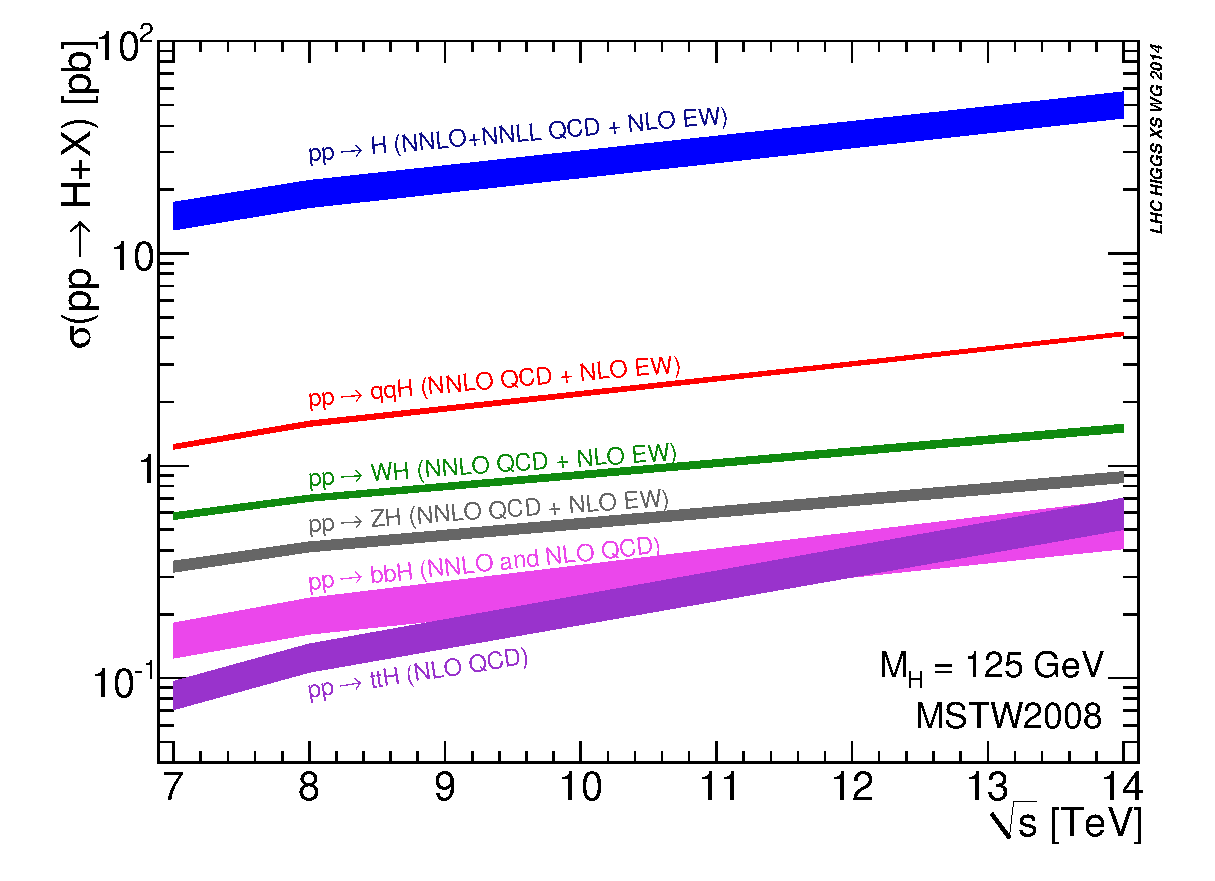
\includegraphics[scale=0.42]{figures/7-14xsec.eps}
\caption{ Higgs boson production cross sections as a function of the centre-of-mass-energies}	
\end{figure}
\end{center}
\end{frame}



\begin{frame}
\frametitle{Branching ratio}
\small{In particle physics, the branching ratio for a decay process is the ratio of the number of particles which decay via a specific decay mode with respect to the total number of particles which decay via all decay modes. \footnotemark.}
\begin{align}
\text{BR} =\frac{\Gamma_i}{\sum_{i}\Gamma_i}
\end{align}
\small{Where $\Gamma=\sum_i\Gamma_i$ is the total decay width (sum of all partial widths) of the particle and is related to lifetime of the particle: $\Gamma=1/\tau$.
Since the dimension of $\Gamma$ is the inverse of time, in our system of natural units, it is measured in inverse seconds} .%it has the same dimension as mass (or energy).}
\footnote[0]{\tiny{Cleaves H.J. (2011) Branching Ratio. In: Gargaud M. et al. (eds) Encyclopedia of Astrobiology. Springer, Berlin, Heidelberg} }
\end{frame}
 
\begin{frame}
\frametitle{Higgs Branching ratio}
\begin{center}
	\begin{figure}
		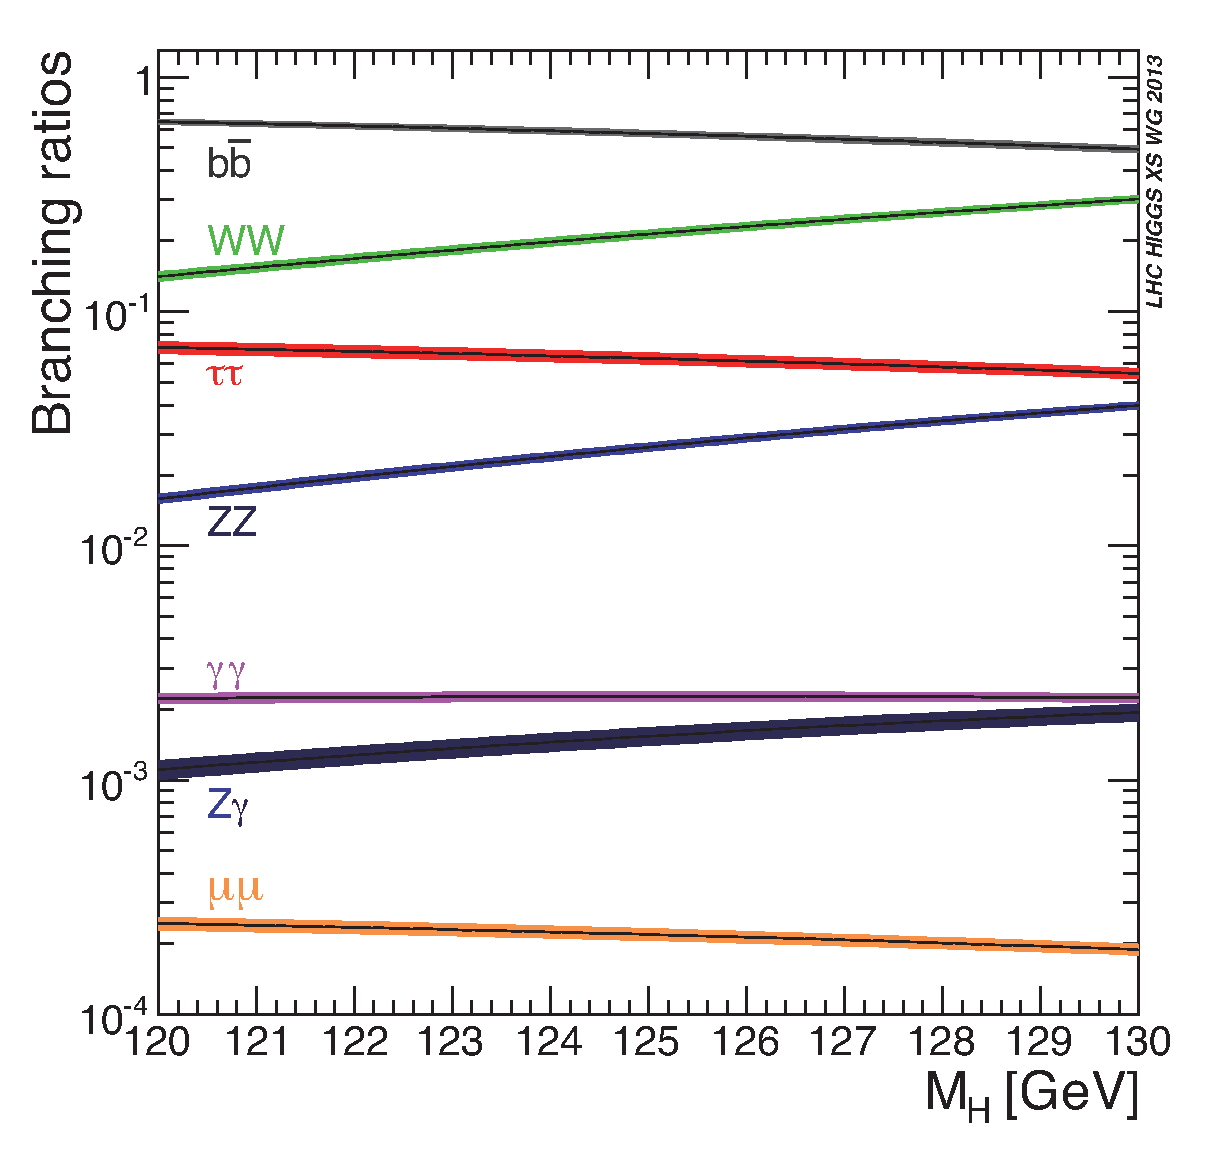
\includegraphics[scale=0.35]{figures/Higgs_BR_120-130_7.eps}
		\caption{Standard Model Higgs boson decay branching ratios}	
	\end{figure}
\end{center}
\end{frame}


\begin{frame}
\section{Higgs Branching ratios }
\frametitle{Higgs Branching ratios per channel}
\begin{table}
	\caption*{SM Higgs boson branching ratios for  $M_H$ =125 GeV}
\begin{center}
\begin{tabular}{|c|c|}
	\hline
	Higgs decay & Branching ratio (BR)\\
	\hline
	H $\rightarrow$ b$\bar{b}$ &
	$50.82\%$ \\
	\hline
	H $\rightarrow$ $W^+W^-$ &
	$21.5\%$ \\
	\hline
	H $\rightarrow$ $\tau^+ \tau^-$ &
	$6.27\%$\\
\hline
	H $\rightarrow$ ZZ &
$2.61\%$\\
\hline
	H $\rightarrow$ $\gamma\gamma$ &
$0.227\%$\\
\hline
	H $\rightarrow$ Z$\gamma$ &
$0.153\%$\\
\hline
	H $\rightarrow$ $\mu^+\mu^-$ &
$0.0217\%$\\
\hline
\end{tabular}
\end{center}
\end{table}

\end{frame}



\begin{frame}
\frametitle{$\mu\mu$ same sign decay rate}
\tiny{Table of decay chains for tH.  Expected number of final events assuming 560 produced tH events.l represents $\mu^{\pm},e^- , \tau^\pm$. }
\begin{table}
\renewcommand{\arraystretch}{0.55}
\begin{tabular}{|p{8cm}|p{1.3cm}|c|}
\hline
Decay chain &BR&Events\\
\hline 
\tiny{$tH \rightarrow$ W$^+$bW$^+$W$^-$ $\rightarrow$ $\mu^+$ $\nu_\mu$b$\mu^+\nu_\mu$  $q \bar{q}'$ } &\tiny{2.096 $\times$10$^{-3}$} &  1.173  \\
\hline
\tiny{$tH \rightarrow $W$^+$bW$^+$W$^-$ $\rightarrow$ $\mu^+\nu_\mu$b$\mu^+\nu_\mu$ $l^- \bar{\nu_l}$ } &\tiny{3.37 $\times$ 10$^{-4}$} &0.899 \\
\hline
\tiny{$tH \rightarrow$ W$^+$b $\tau^+ \tau^-$ $\rightarrow$ $\mu^+ \nu_\mu$ b $ \mu^+ \nu_\mu \bar{\nu_\tau} l^-\bar{\nu_l} \nu_\tau$} &\tiny{3.637$\times$10$^{-4}$}&0.203 \\
\hline
\tiny{$tH \rightarrow$ W$^+$bW$^+$W$^-$ $\rightarrow$ $\tau^+ \bar{\nu_\tau}$b $\mu^+ \nu_\mu$  $q\bar{q}$ $\rightarrow$ $\mu^+ \nu_\mu$ $\bar{\nu_\tau}$ $\bar{\nu_\tau}$ b$\mu^+ \nu_\mu$  $q \bar{q}$} &\tiny{1.890$\times$10$^{-4}$}&0.105  \\
\hline
\tiny{$tH \rightarrow$ W$^+$b $\tau^+ \tau^-$ $\rightarrow$ $\mu^+$ $\nu_\mu$b $\nu_\tau$ $\mu^+$ $\nu_\mu \bar{\nu_\tau}$} $q \bar{q}$  &
\tiny{1.681 $\times$10$^{-4}$} & 0.094 \\
\hline
\tiny{$tH \rightarrow$ W$^+$b W$^+$W$^-$ $\rightarrow$ $\tau^+ \bar{\nu_\tau}$b$ \mu^+ \nu_\mu l^- \bar{\nu_l}$ $\rightarrow$ $\mu^+\nu_\mu$ $ \bar{\nu_\tau} \bar{\nu_\tau}$  b$ \mu^+ \nu_\mu l^- \bar{\nu_l}$} &\tiny{3.045$\times$10$^{-5}$}& 0.017\\
\hline
\tiny{$tH \rightarrow$ W$^+$bZZ $\rightarrow$ $q \bar{q}$bZZ $\rightarrow$ $q \bar{q} $ b $\mu^+ \mu^- \mu^+ \mu^-$} & \tiny{1.966$\times$10$^{-5}$} &0.011\\
\hline 
\tiny{$tH \rightarrow$ W$^+$b $\tau^+ \tau^-$ $\rightarrow$ $\tau^+ \bar{\nu_\tau}b$ $\mu^+ \nu_\mu \bar{\nu_\tau} $  $q\bar{q}' \nu_\tau$ $\rightarrow$  $\mu^+ \nu_\mu \bar{\nu_\tau}\bar{\nu_\tau} $b $\mu^+ \nu_\mu \bar{\nu_\tau} $  $q\bar{q}' \nu_\tau$ } &\tiny{1.549 $\times$10$^{-5}$} &  0.008  \\
\hline
%\tiny{$tH \rightarrow$W$^+$bZ$\gamma$ $\rightarrow$ $\mu^+ \nu_\mu$ b $\mu^+ \mu^- \gamma$} & \tiny{6.888$\times$10$^{-6}$}&0.003\\
%\hline 
%\tiny{$tH \rightarrow$W$^+$bZZ $\rightarrow$ $\mu^+ \nu_\mu$ b $\mu^+ \mu^- l^+l^-$} &\tiny{3.962$\times$10$^{-6}$ }&0.002\\
%\hline 
%%\tiny{$tH \rightarrow$ $\tau \nu_\tau $bZ$\gamma$ $\rightarrow$ $\mu^- \bar{\nu_\mu} \nu_\tau \nu_\tau$ b $\mu^+ \mu^- \gamma$} & 6.347$\times$10$^{-7}$ & 0.0003\\
%%\hline 
\end{tabular}
\end{table}
\end{frame}

\begin{frame}
\frametitle{LHC}
\begin{center}
	\begin{figure}
	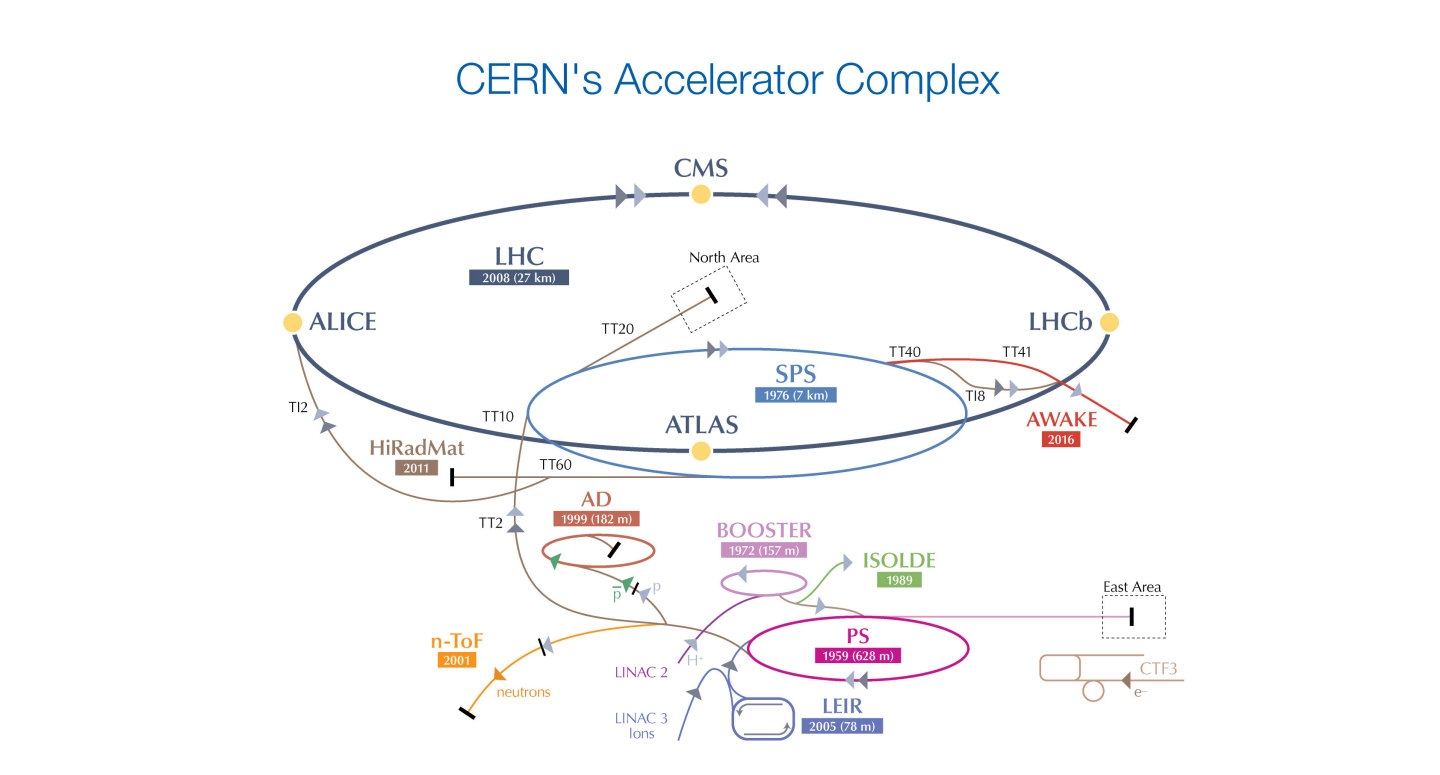
\includegraphics[scale=0.25]{figures/CERN's-accelerator-complex2013.jpg}
	\end{figure}
\end{center}
\end{frame}



\begin{frame}
\frametitle{LHC parameters}
\begin{center}
	\begin{figure}
		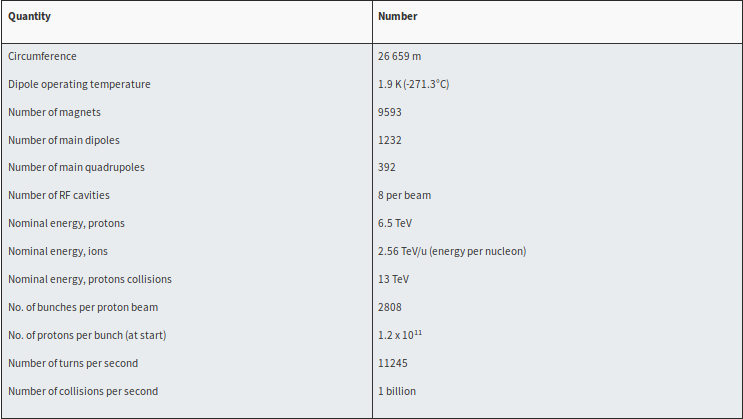
\includegraphics[scale=0.5]{figures/lhc-t.png}
		\caption*{Table. LHC characteristics for run 2.}
	\end{figure}
\end{center}
\end{frame}


\begin{frame}
\frametitle{LHC}
\begin{table}
	\caption*{Accelerator operation energies}
	\begin{tabular}{|c|c|}
		\hline
		Accelerator & Energy \\
		\hline
		Linac 2 &  50 MeV \\
		\hline
		PS Booster & 1.4 GeV \\
		\hline
		Proton Scyncroton (PS) & 25 GeV\\
		\hline
		SPS &  450 GeV\\
		\hline
		LHC & 6.5 TeV\\
		\hline
	\end{tabular}
\end{table}
\end{frame}

\begin{frame}
\frametitle{CMS detector}
\begin{center}
	\begin{figure}
		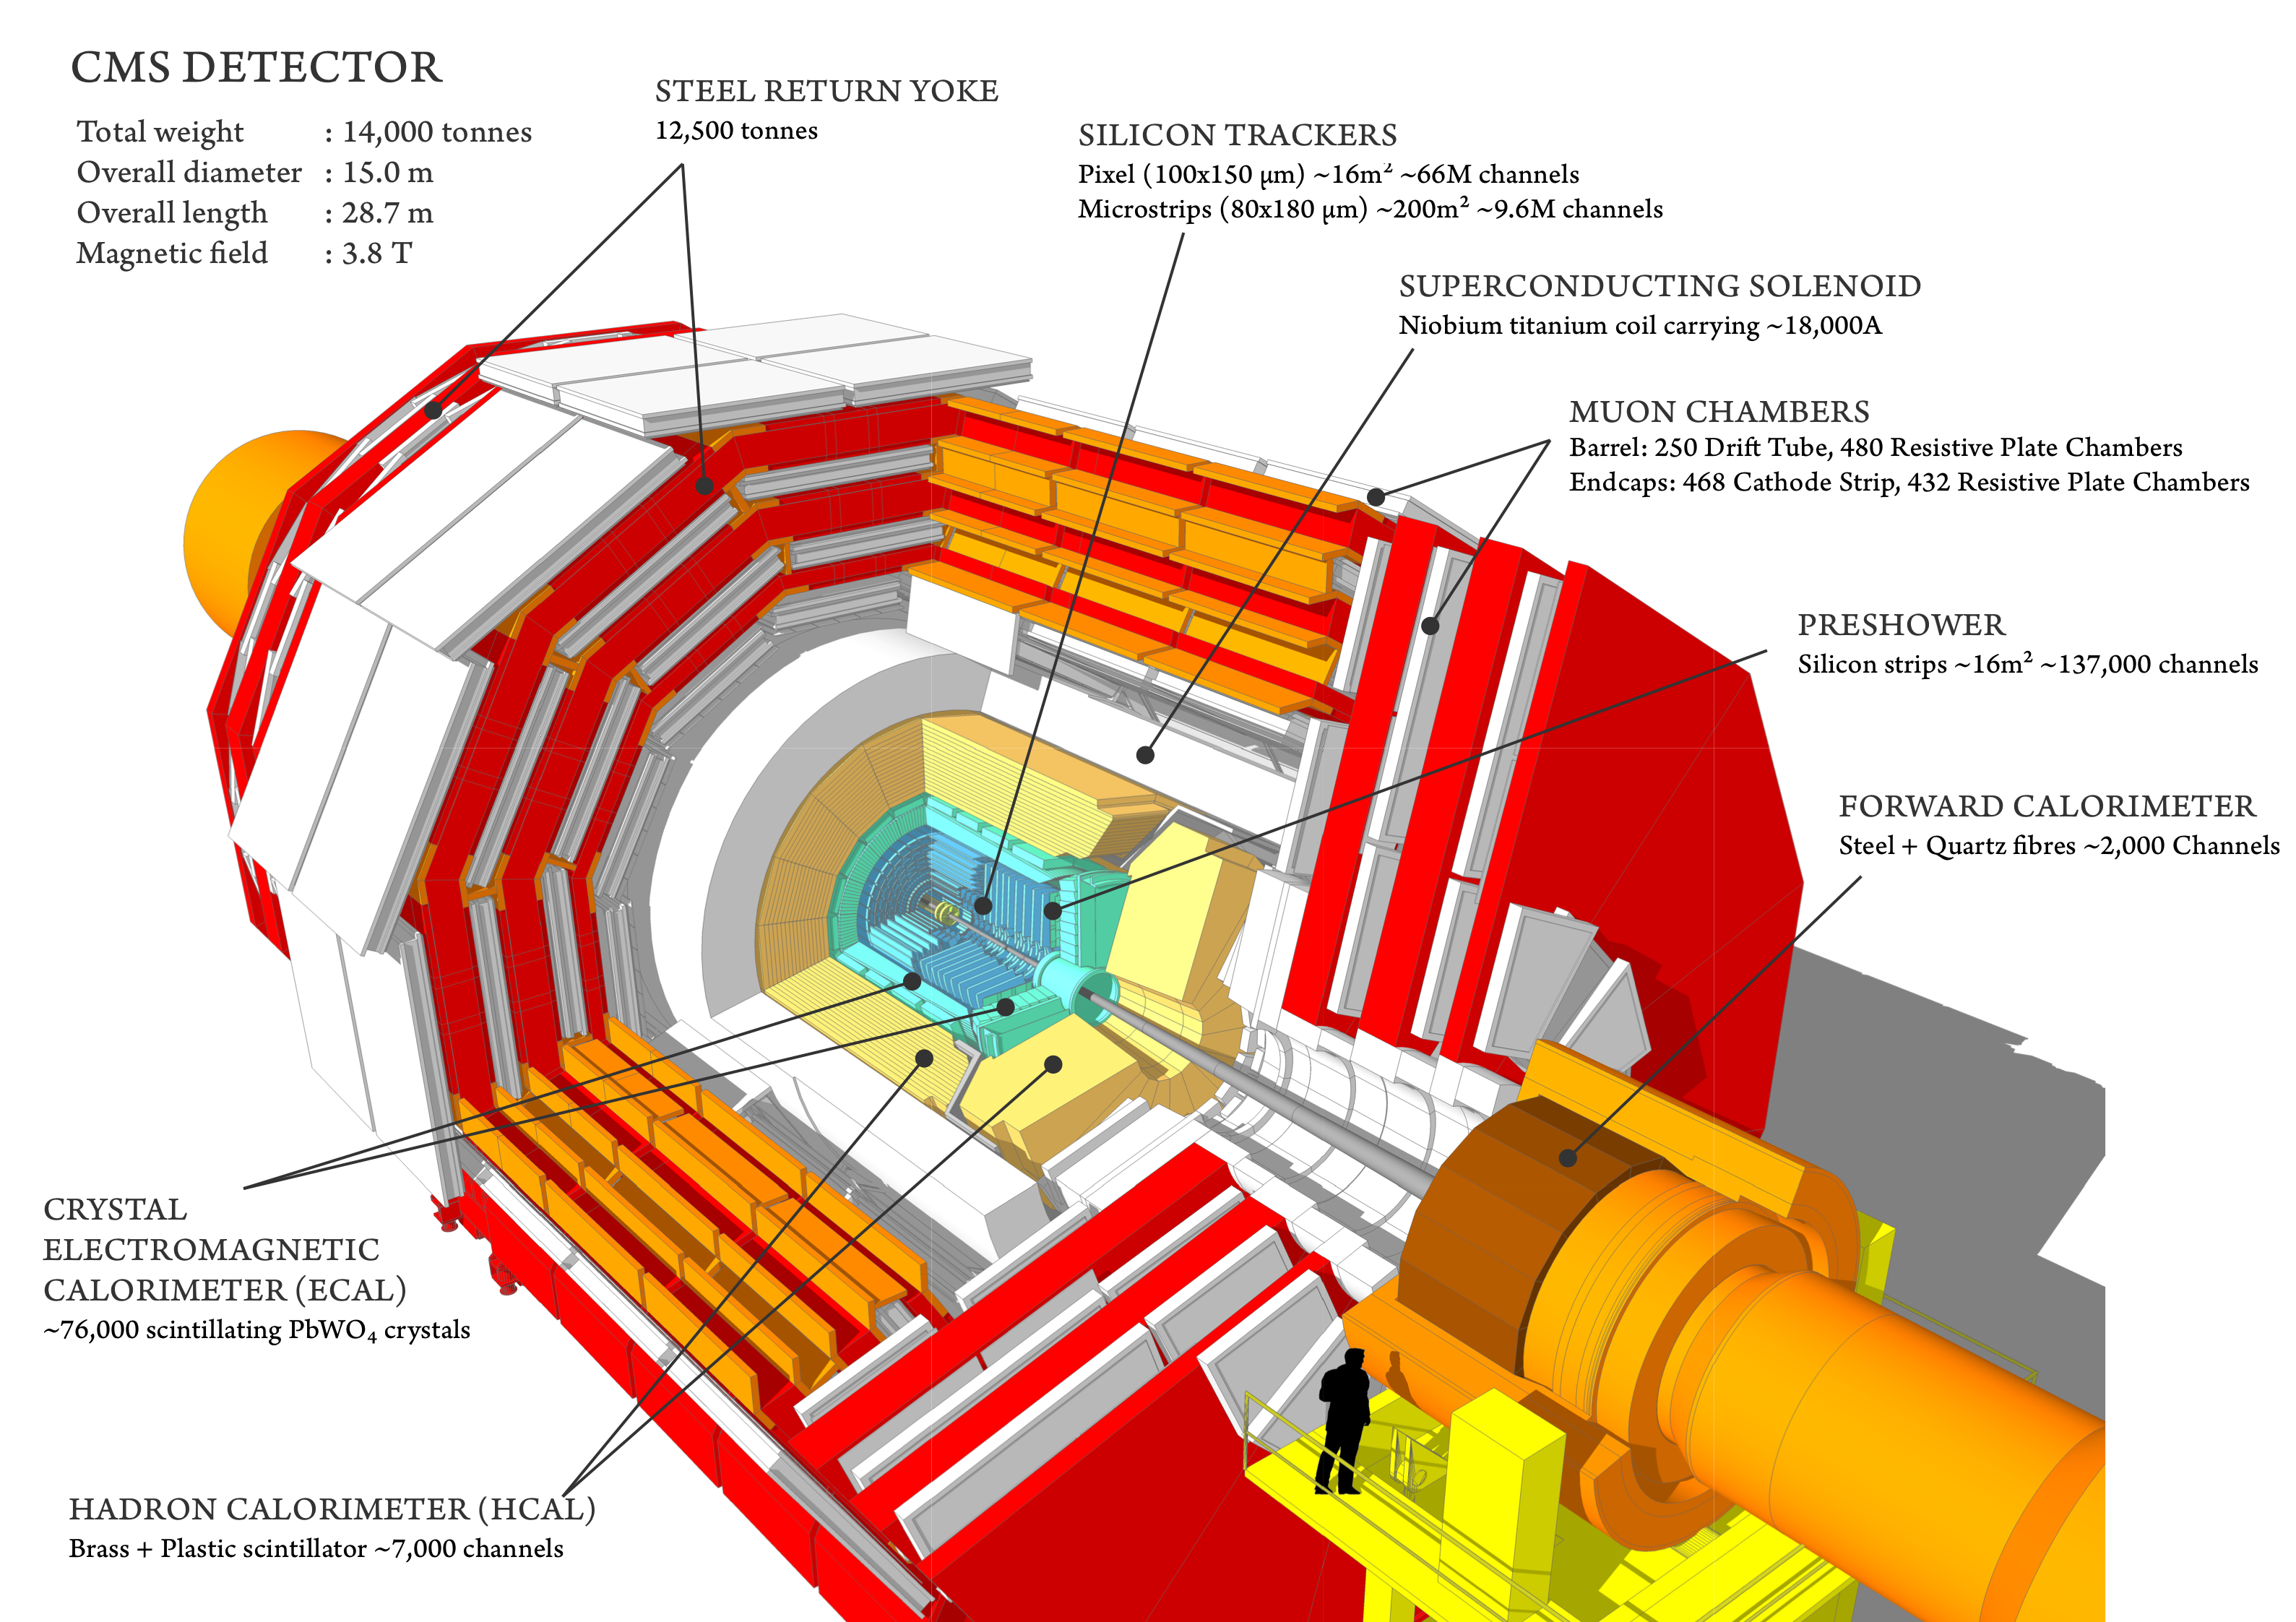
\includegraphics[scale=0.08]{figures/cms.png}
		\caption{Compact muon solenoid}
	\end{figure}
\end{center}
\end{frame}

\begin{frame}
\frametitle{CMS integrated luminosity}
\begin{center}
	\begin{figure}
		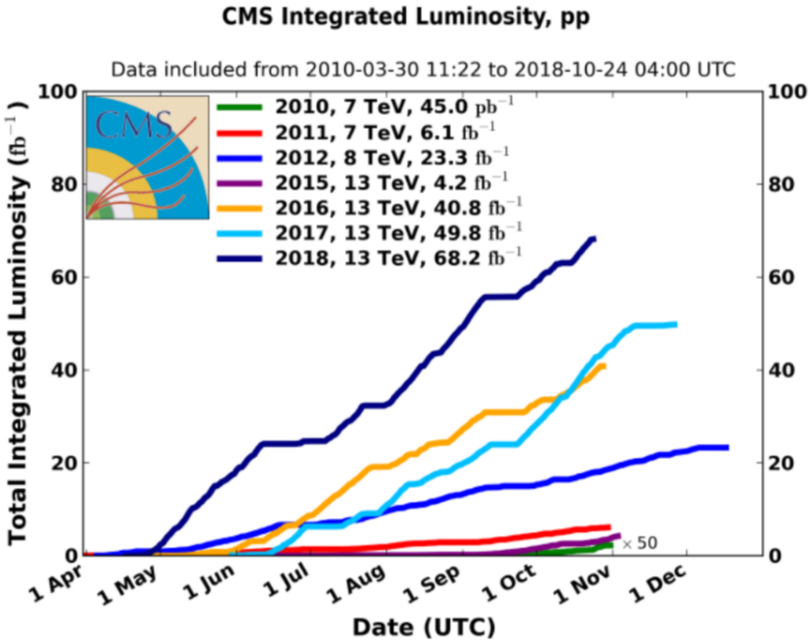
\includegraphics[scale=0.23]{figures/cms_lumi.png}
		\caption{Integrated luminosity for CMS experiment }
	\end{figure}
\end{center}
\end{frame}




\begin{frame}
\frametitle{Topology of events tH}
The characteristics of the signal tH:

\begin{multicols}{2}
\tiny{
\begin{itemize}
\item t$\rightarrow$W$^+$b$\rightarrow$ $l^+ \nu_\mu$b
\item H$\rightarrow$ W$^+$W$^-$ 

\begin{list}{--}{}
\item  \tiny{W$\rightarrow$ $l^\pm \nu$, where l can be $\mu^\pm$,$e^-$  $\tau^\pm$} 
\item   \tiny{W$\rightarrow$ q$\bar{q}$}
\item \tiny{W bosons decay leptonically resulting in a signature of two same-sign leptons }
\end{list}
\item a light-flavor quark 
\item  b quark jet  \cite{2}
\end{itemize}
}
\columnbreak
\begin{figure}
	\centering
	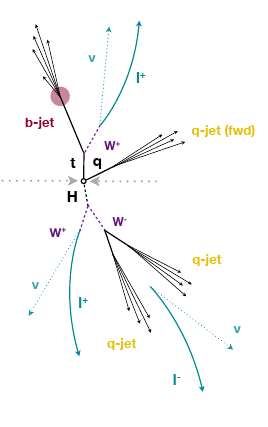
\includegraphics[scale=0.5]{figures/jet.png}
\end{figure}
\end{multicols}
\end{frame}

\begin{frame}
\frametitle{Event selection}
The main analysis strategy is to obtain a selection of events compatible with
certain characteristics of the signal at pre-selection level.\\

It is required:
\begin{itemize}
\item The events are selected those that contain two leptons ($l^+l^-$)  with the same sign.
\item Transverse moment $p_{t}$ > 25 and 15 GeV, for the muons.
\item A foward jet with $p_t$ > 40 GeV, | $\eta$ | > 2.4
\item One or more b-jets with (| $\eta$ | <2.4)\cite{1}
\end{itemize}
\end{frame}

\begin{frame}
\section{Previous results}
\frametitle{Previous results}
\begin{itemize}
\item Direct searches for tHq production using all relevant Higgs decay modes
have previously been carried out by CMS in the 8 TeV dataset in pp collisions\cite{5} 
\item On 2015, in pp collisions with $\sqrt{s}$=13 TeV data set using the H$\rightarrow$b$\bar{b}$ channel, corresponding to an
integrated luminosity of 35.9 fb$^-1$\cite{6}
\item In 2016, for $\sqrt{s}$= 13 TeV dataset, a search for t$\bar{t}$H production in multilepton
final states recently produced first evidence for associated production of top quarks and Higgs
bosons\cite{2}
\end{itemize}
\end{frame}

\begin{frame}
\frametitle{Previous results for t$\bar{t}$H production}
\begin{multicols}{2}
\begin{center}
	\begin{figure}
		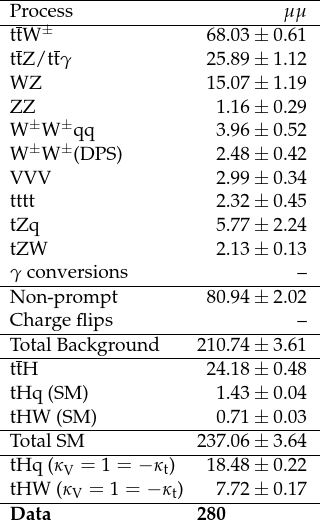
\includegraphics[scale=0.4]{figures/tth-table.png}
		\caption*{}
	\end{figure}
\end{center}
\columnbreak
\begin{center}
	\begin{figure}
		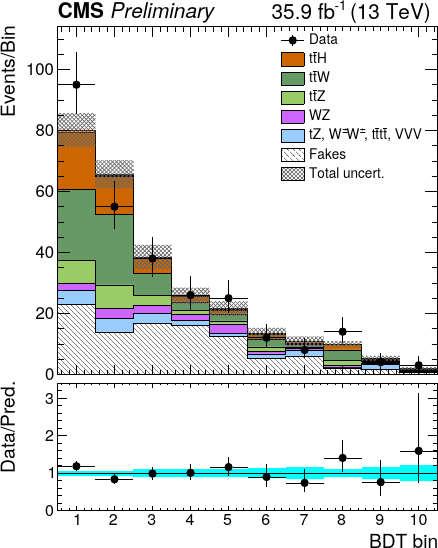
\includegraphics[scale=0.3]{figures/bdt.png}
		\caption*{\tiny{Post-fit categorized BDT classifier outputs as used in
			the maximum likelihood fit for the $\mu\mu$ channel for
			35.9 fb$^{-1}$.In the box below each distribution, the ratio
			of the observed and predicted event yields is shown.\cite{2}
		 }}
	\end{figure}
\end{center}
\end{multicols}
\end{frame}

\begin{frame}
	\begin{center}
		\begin{figure}
			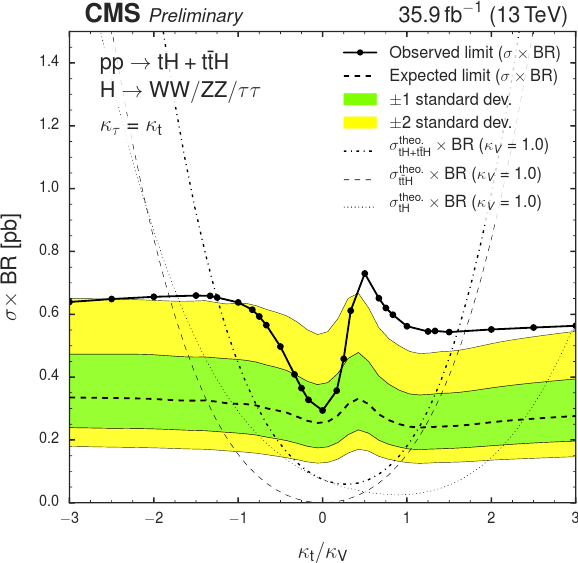
\includegraphics[scale=0.3]{figures/sc.png}
			\caption{Observed and expected 95$\%$ C.L. upper limit on the tH + t$\bar{t}$H cross section times H $\rightarrow$ WW $+$ $\tau\tau$ $+$ ZZ branching fraction for different 20 values of the coupling ratio $\kappa_t /\kappa_v$ . The expected limit is derived from a background-only MC dataset.}
		\end{figure}
	\end{center}
\end{frame}


\begin{frame}
\frametitle{Main backgrounds}
In the leptonic channels, the main backgrounds are expected to
	arise from the production of top quarks
	\begin{itemize}
	\item In the dominant t$\bar{t}$ mode, where 
 same-sign dilepton signatures can occur when a non-prompt lepton from heavy-flavor
decay passes the signal selection, or in associated production with a W/Z or Higgs boson.
	\item Processes with single top quarks also contribute, mostly in the associated production with a Z
	boson (tZ) or when produced with both a W and a Z boson (WZ) 

\end{itemize}
\end{frame}

\begin{frame}
\frametitle{Main backgrounds}
\begin{itemize}
\item t$\bar{t}$W$^\pm$ and t$\bar{t}$Z (t$\bar{t}$V): Backgrounds are estimated directly from simulated events% which are corrected for data/MC differences and
	%inefficiencies in the same way as signal events. 
	\item WZ: Diboson production with leptonic Z decays and additional jet radiation in the final state can
	lead to signatures very similar to that of the signal. Due to the larger cross section, the main
	contribution arises from WZ production.
	\item t$\bar{t}$H: tHq production which decays to same sign deleptons.
\item Rare SM (tZ,VVV,WW,tttt): Due to small event yields, all these process are grouped as one.
\item Non prompt leptons b quark decays and spurious lepton signatures from hadronic jets.
\end{itemize}
\end{frame}

\begin{frame}
\frametitle{Main backgrounds}
\begin{tabular}{|c|c|c|}
	Background & $\sigma$[pb] & Decay process \\
	\hline
t$\bar{t}$H	& 0.2151 & W$^+$b W$^+$b WW $\rightarrow$ $\mu \nu_\mu$b$\mu \nu_\mu$b $\mu^+\mu^-$$\mu^+\mu^-$\\
\hline  
t$\bar{t}$W$^\pm$ and &0.2043 &  W$^+$b W$^+$b$\mu^+\mu^-$\\
\hline
 t$\bar{t}$Z & 0.2529 & \\
 \hline 
  WW  &1.64 & $\mu^+ \mu^- \mu^+ \mu^-$\\
    \hline 
  tZq  &0.0758 & tZq$\rightarrow$  $\mu^+$ $\nu_\mu$b$ \mu^+ \mu^-$q \\
    \hline 
  tttt  & 0.0091&W$^+$bW$^+$bW$^+$bW$^+$bW$^+$b $\rightarrow$  $\mu^+$ $\nu_\mu$b $\mu^+$ $\nu_\mu$b  $l^+$ $\nu_l$b $l^+$ $\nu_l$b \\
    \hline 
  wwz  & 0.1651& $\mu^+ \mu^- \mu^+ \mu^- l^+l^-$\\
    \hline 
  zzz  &0.1396 &$\mu^+ \mu^-\mu^+ \mu^- l^+l^- $  \\
    \hline 
  wzz  & 0.0556&$\mu^+ \mu^-\mu^+ \mu^-  l^+l^-$  \\
  \hline 
 WZ &4.42965 &$\mu^+ \mu^-\mu^+ \mu^-$ \\
 \hline
ZZ &  1.256 & $\mu^+ \mu^-\mu^+ \mu^-$ \\
 \hline
\end{tabular}


\end{frame}

\begin{frame}
\frametitle{Boosted decision tree (BDT)}
\begin{itemize}
\item A decision tree takes a set of input features and splits input data recursively based on
those features.
Boosting is a method of combining many weak learners (trees) into a strong classifier. The features can be a mix of categorical and continuous data.
\item The BDT training is performed using several event variables for signal and background. 
	\item BDT training uses MC samples for  t$\bar{t}$W$^\pm$ and t$\bar{t}$Z (t$\bar{t}$V),
	because t$\bar{t}$V is one of the biggest backgrounds
\end{itemize}
\end{frame}


\begin{frame}
\frametitle{BDT Variables}
\begin{itemize}
\item	Trailing lepton $p_{t}$
\item 	Total charge of tight leptons
\item 	min $\Delta$R (lepton pairs)
\item 	$\Delta\phi$ between highest $p_t$ lepton pair
\item 	Number of jets with |$\eta$| < 2.4
\item	Number of non b-tagged jets with |$\eta$| > 1.0
\item	Maximum |$\eta$| for jets
\item	$\Delta\eta$ (most forward light jet, closest lepton)
\item	$\Delta\eta$ (most forward light jet, hardest loosely b-tagged jet)
\item	$\Delta\eta$ (most forward light jet, 2nd hardest loosely b-tagged jet)
\end{itemize}
\end{frame}

\begin{frame}
\frametitle{Sources of uncertainty on event yields}
\begin{itemize}
\item Luminosity measurement: ~2.6$\%$.
\item Data/MC scale factors for lepton selection (ID, iso) and trigger efficiencies ~5$\%$ per lepton.
\item Choice of PDF set:
\begin{itemize}
 \item 3.7$\%$ for tHq
 \item ~4$\%$ for tHW t$\bar{t}$W, t$\bar{t}$Z, t$\bar{t}$H 
 \item Scale uncertainties: 12$\%$, 4 for t$\bar{t}$W, 10$\%$ for t$\bar{t}$Z, +5.8/-9.2$\%$ for t$\bar{t}$H.
\end{itemize}
 \item Background: WZ, ZZ sample modelling and statistics: ~50$\%$.
 \item Rare SM (tZ,tri-bosons, WWqq, tttt) : 50$\%$
 \item Fake rate estimation:
 The predicted event yield has a normalization uncertainty of ~30-50$\%$ \cite{7}
\end{itemize}

\end{frame}


\begin{frame}
\frametitle{Uncertainty values}
Common uncertainties for MC :
\begin{itemize}
	\item Muon identificacion 6$\%$
	\item Dimuon Trigger  1$\%$ 
\end{itemize}
\begin{table}
			\renewcommand{\arraystretch}{0.1}
	\begin{tabular}{|c|M{2.7cm}|M{2.3cm}|}
\hline
\scriptsize{Background}& \scriptsize{Sources of systematic uncertainty}& \scriptsize{Total Systematic Uncertainty} \\
\hline
\rule{0pt}{3pt}t$\bar{t}$H  &{\begin{itemize} \tiny{ 
 	\item PDF 4$\%$ \\
 	\item QCD scale 5.8$\%$ \\
 	\item Higgs BR  1$\%$ }
\end{itemize}}  & 9.36$\%$ \\
 \hline  
 t$\bar{t}$Z&{\begin{itemize} \tiny{ 
 			\item PDF 4$\%$ \\
 			\item QCD scale 10$\%$ \\
 			 }
 \end{itemize}} & 12.36 $\%$ \\
 \hline
 t$\bar{t}$W&{\begin{itemize} \tiny{ 
 			\item PDF 4$\%$ \\
 			\item QCD scale 12$\%$ \\
 		}
 \end{itemize}} &14.03 $\%$ \\
 \hline
\end{tabular}
\end{table}
\end{frame}

\begin{frame}
\begin{table}
		\renewcommand{\arraystretch}{0.1}
	\begin{tabular}{|c|M{2.7cm}|M{2.3cm}|}
\hline
\scriptsize{Background}& \scriptsize{Sources of systematic uncertainty}& \scriptsize{Total Systematic Uncertainty} \\
		\hline
	 \tiny{Rares SM} & {\begin{itemize} \tiny{
				\item Rare SM 50$\%$ }
	\end{itemize}}&50.36 $\%$ \\
	\hline
	\tiny{WZ} & {\begin{itemize}\tiny{
				\item Sample modelling and statistics 50$\%$ }
	\end{itemize}} & 50.36$\%$ \\
	\hline 
	\tiny{Non prompt leptons} &{\begin{itemize} \tiny{
				\item Fake rate estimation 50$\%$
				\item Closure 7$\%$ }
	\end{itemize}} 		 & 50.48$\%$ \\
	\hline 
	\end{tabular}
\end{table}

\end{frame}




\begin{frame}
\section{Fitting}
\frametitle{Fitting}
	\begin{center}
	\begin{figure}
		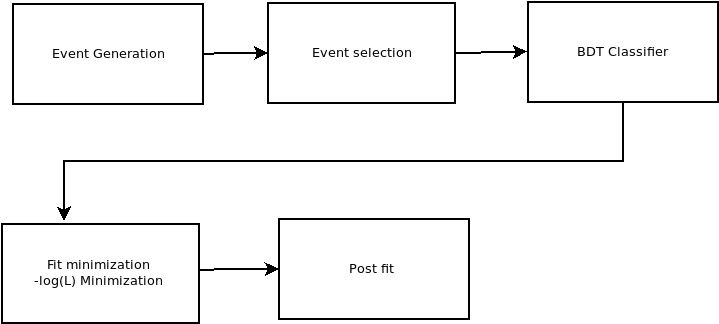
\includegraphics[width=10.5cm]{figures/fit-box.png}
		\caption*{}
	\end{figure}
\end{center}
\end{frame}

\begin{frame}
\frametitle{Likelihood model}
The likelihood function is the product of Poisson probabilities for all bins
\begin{align}
L(\mu,\theta)=\prod_{j=1}^{N}\frac{(\mu s_j +b_j)^{n_j}}{n_j !}e^{-(\mu s_j+b_j)}
\end{align}

\begin{itemize}
	\item	N=number of bins
	\item	$\mu$=parameter of signal
	\item	s=signal
	\item	b=background
	\item	n=number of events
\end{itemize}
\end{frame}


\begin{frame}
\section{Results}
\frametitle{Results}

\begin{table}
	\caption{Prefit and postfit table for each yield.}
\begin{tabular}{|c|c|c|}
	\hline
	Process  & Number of events prefit    & Number of events Postfit \\
	\hline
	tH & 2.13 $\pm$ 0.21  & 5.36$\pm$27.40\\
	\hline
	t$\bar{t}$H  &  24.18 $\pm$ 2.26 & 24.81 $\pm$ 2.24 \\
	\hline
	t$\bar{t}$W  &  68.03 $\pm$ 9.54 & 77.01 $\pm$ 8.76\\
	\hline
	t$\bar{t}$Z  & 25.89 $\pm$ 3.20 & 26.74 $\pm$ 3.18\\
	\hline
	Rares SM & 17.17 $\pm$ 8.64 & 18.77 $\pm$ 8.66\\
	\hline
	WZ & 16.23 $\pm$ 8.17 & 17.41 $\pm$ 8.04\\
	\hline
	fakes  & 80.94 $\pm$ 40.86  & 100.15 $\pm$ 29.30\\
	\hline
\end{tabular}	
\end{table}
 Prefit uncertainty is statistical only. Postfit uncertainty is statistical + systematic.
\end{frame}


\begin{frame}
\frametitle{Results}
\begin{minipage}{0.5\textwidth}
	\begin{center}
	\begin{figure}
		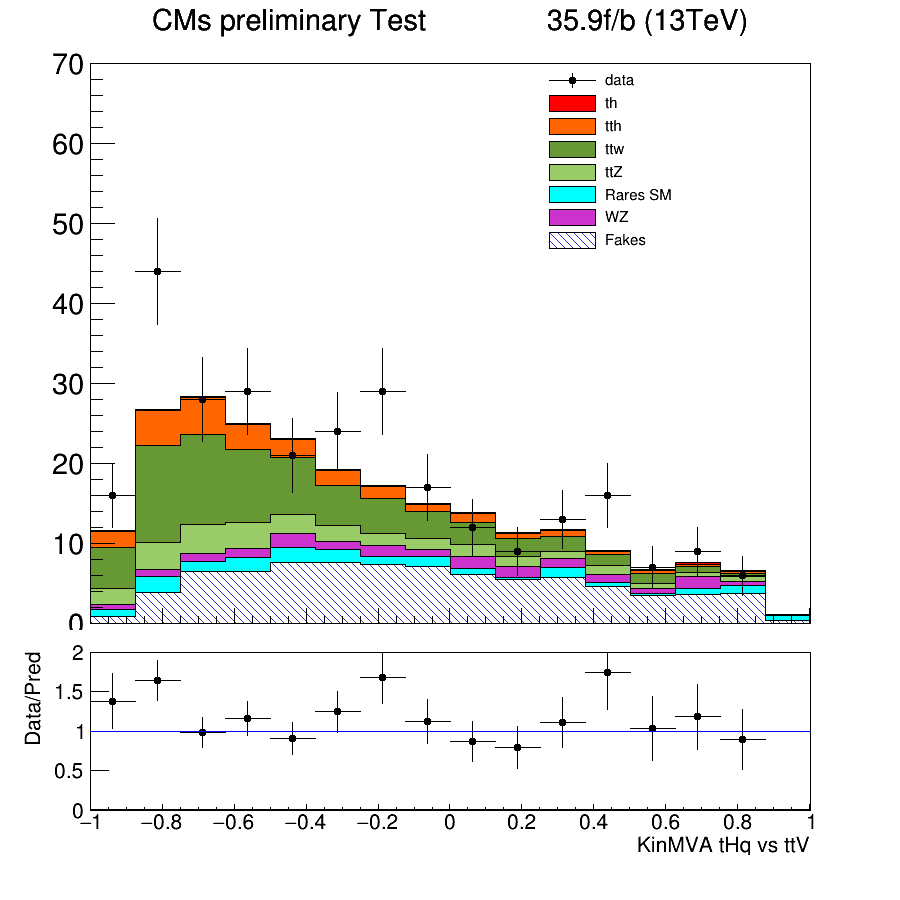
\includegraphics[width=6cm,height=5cm]{figures/kin.png}
		\caption*{\tiny{Pre-fit signal and background yields for tH process. In the
			box below each distribution, the ratio of the observed and predicted event yields is shown}}
	\end{figure}
\end{center}
\end{minipage}\hfill
\begin{minipage}{0.5\textwidth}
	\begin{center}
	\begin{figure}
		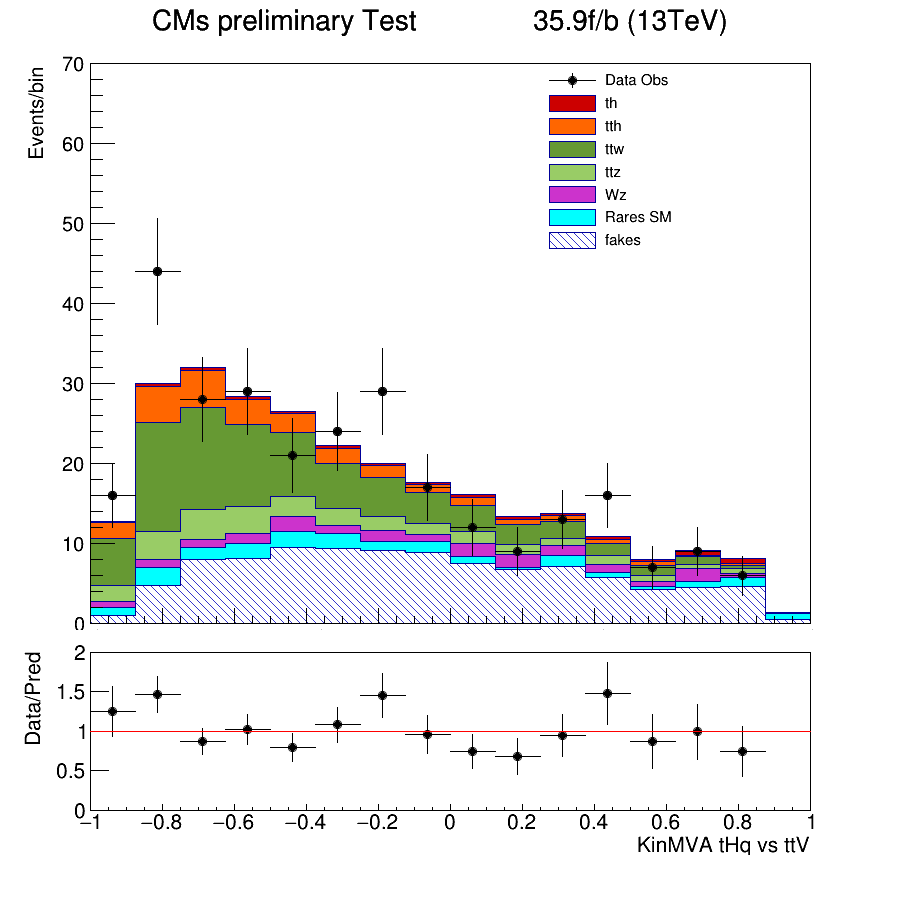
\includegraphics[width=6cm,height=5cm]{figures/simple.png}
		\caption*{\tiny{Post-fit signal and background yields for tH process. In the
			box below each distribution, the ratio of the observed and predicted event yields is shown}}
	\end{figure}
\end{center}
\end{minipage}
\end{frame}

\begin{frame}
\frametitle{Results}

\begin{table}
\caption{Prefit and postfit table for each yield. $k_{t}$ =-1.}
	\begin{tabular}{|c|c|c|}
		\hline
		Process  & Number of events prefit    & Number of events Postfit \\
		\hline
		tH & 26.2 $\pm$2.60 & 1.83 $\pm$ 26.63\\
		\hline
		t$\bar{t}$H  & 24.18 $\pm$ 2.26& 24.82 $\pm$ 2.27\\
		\hline
		t$\bar{t}$W  & 68.03  $\pm$ 9.54 & 77.07 $\pm$ 8.99\\
		\hline
		t$\bar{t}$Z  & 25.89  $\pm$  3.20& 26.76 $\pm$ 3.18\\
		\hline
		Rares SM & 17.17  $\pm$ 8.64 & 18.90 $\pm$ 8.37\\
		\hline
		WZ & 16.23  $\pm$ 8.17& 17.54 $\pm$ 8.15\\
		\hline
		fakes  & 80.94   $\pm$ 40.86& 102.97 $\pm$ 29.51\\
		\hline
	\end{tabular}	
\end{table}
 Prefit uncertainty is statistical only. Postfit uncertainty is statistical + systematic.
\end{frame}


\begin{frame}
\frametitle{Results}
\begin{minipage}{0.5\textwidth}
	\begin{center}
		\begin{figure}
			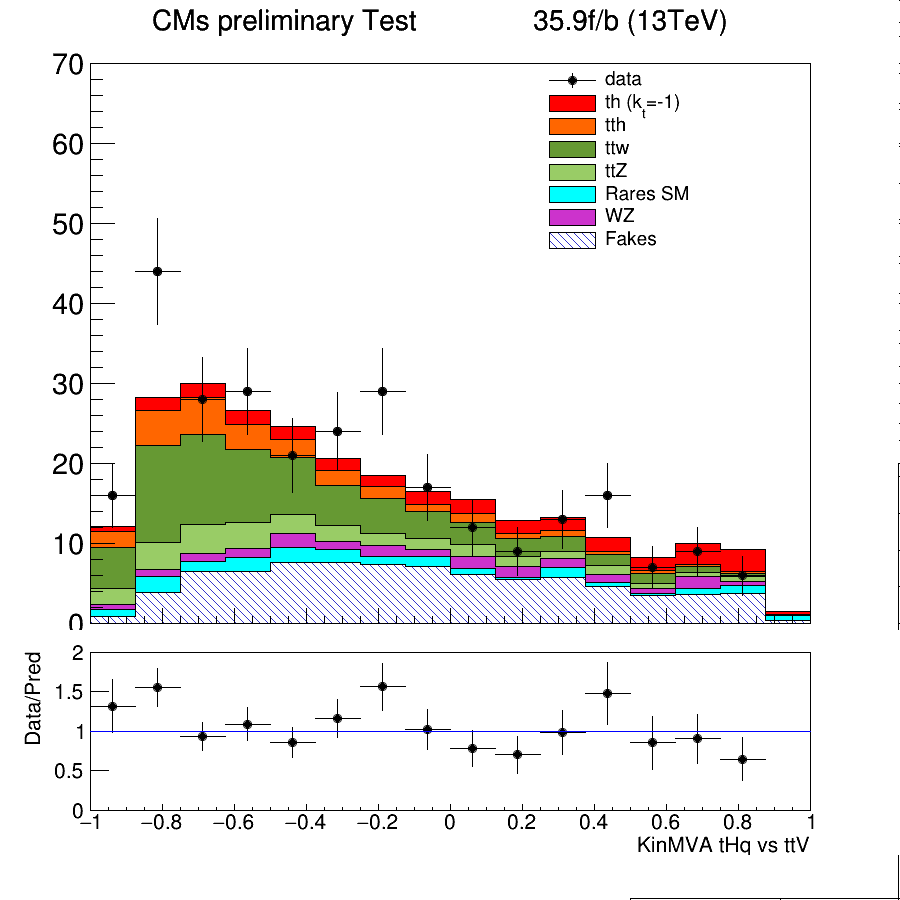
\includegraphics[width=6cm,height=5cm]{figures/kin-kt-1.png}
			\caption*{\tiny{Pre-fit signal and background yields for tH process for $k_t$=-1.\\
					 In the box below each distribution, the ratio of the observed and predicted event yields is shown}}
		\end{figure}
	\end{center}
\end{minipage}\hfill
\begin{minipage}{0.5\textwidth}
	\begin{center}
		\begin{figure}
			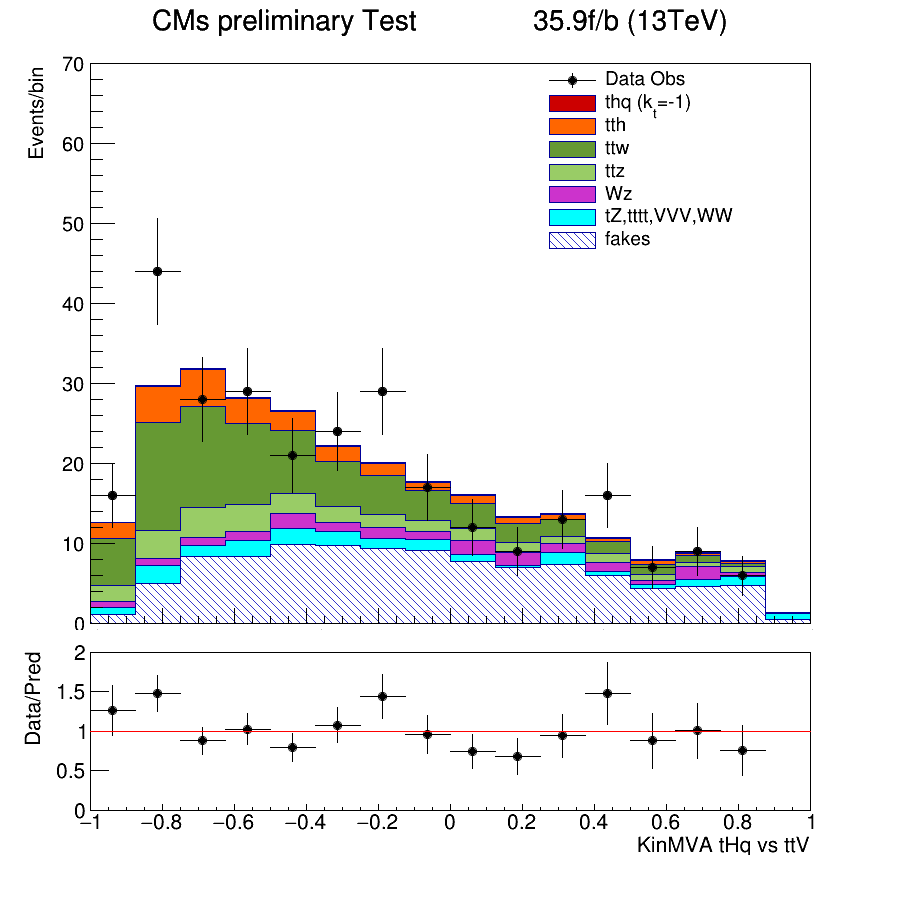
\includegraphics[width=6cm,height=5cm]{figures/simple-kt-1.png}
			\caption*{\tiny{Post-fit signal and background yields for tH process for $k_t$=-1. \\ In the
					box below each distribution, the ratio of the observed and predicted event yields is shown}}
		\end{figure}
	\end{center}
\end{minipage}
\end{frame}




\begin{frame}
\frametitle{Results}
\framesubtitle{Likelihood scan}
To test a hypothesized value of $\mu$ we consider the profile likelihood ratio
\begin{align}
\lambda(\mu)=\frac{L(\mu,\hat{\hat{\theta}})}{L(\hat{\mu},\hat{\theta})}
\end{align}
\small{
\begin{itemize}
\item Here $\hat{\hat{\theta}} $ in the numerator denotes the value of $\theta$ that maximizes L for the specified $\mu$,
it is the conditional maximum-likelihood (ML) estimator of $\hat{\theta}$ (and thus is a function of $\mu$).
The denominator is the maximized (unconditional) likelihood function, i.e., $\hat{\mu}$ and $\hat{\theta}$ are
their ML estimators\cite{3}. 
\item The presence of the nuisance parameters broadens the profile likelihood as a
function of $\mu$ relative to what one would have if their values were fixed. This reflects the loss
of information about $\mu$ due to the systematic uncertainties\cite{3}\cite{4}. 
\end{itemize}
}
\end{frame}


\begin{frame}
\frametitle{Results}
\framesubtitle{Likelihood scan}
\begin{minipage}{0.5\textwidth}
	\begin{center}
		\begin{figure}
			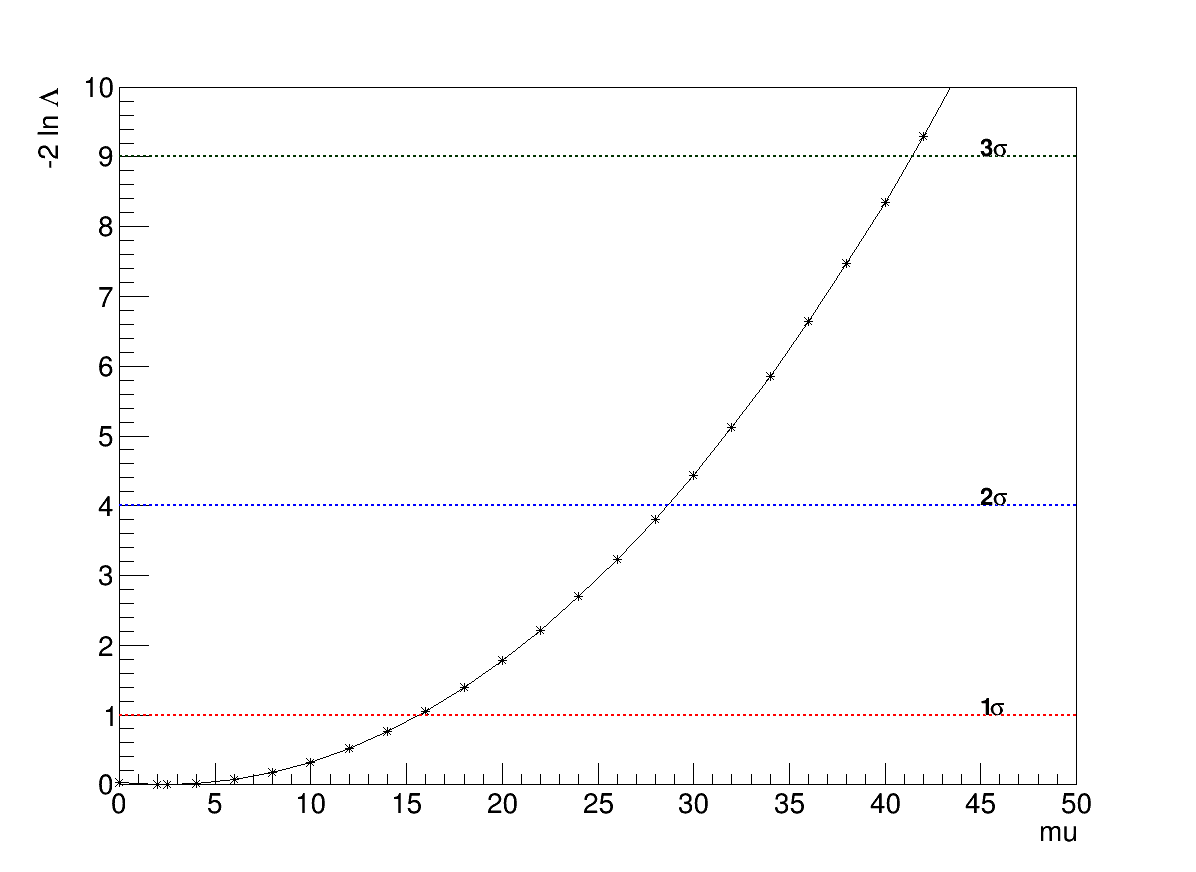
\includegraphics[width=6cm,height=5cm]{figures/Likelihood.png}
			\caption*{Likelihood scan for k$_t$=1 (SM)}
		\end{figure}
	\end{center}
\end{minipage}\hfill
\begin{minipage}{0.5\textwidth}
	\begin{center}
		\begin{figure}
			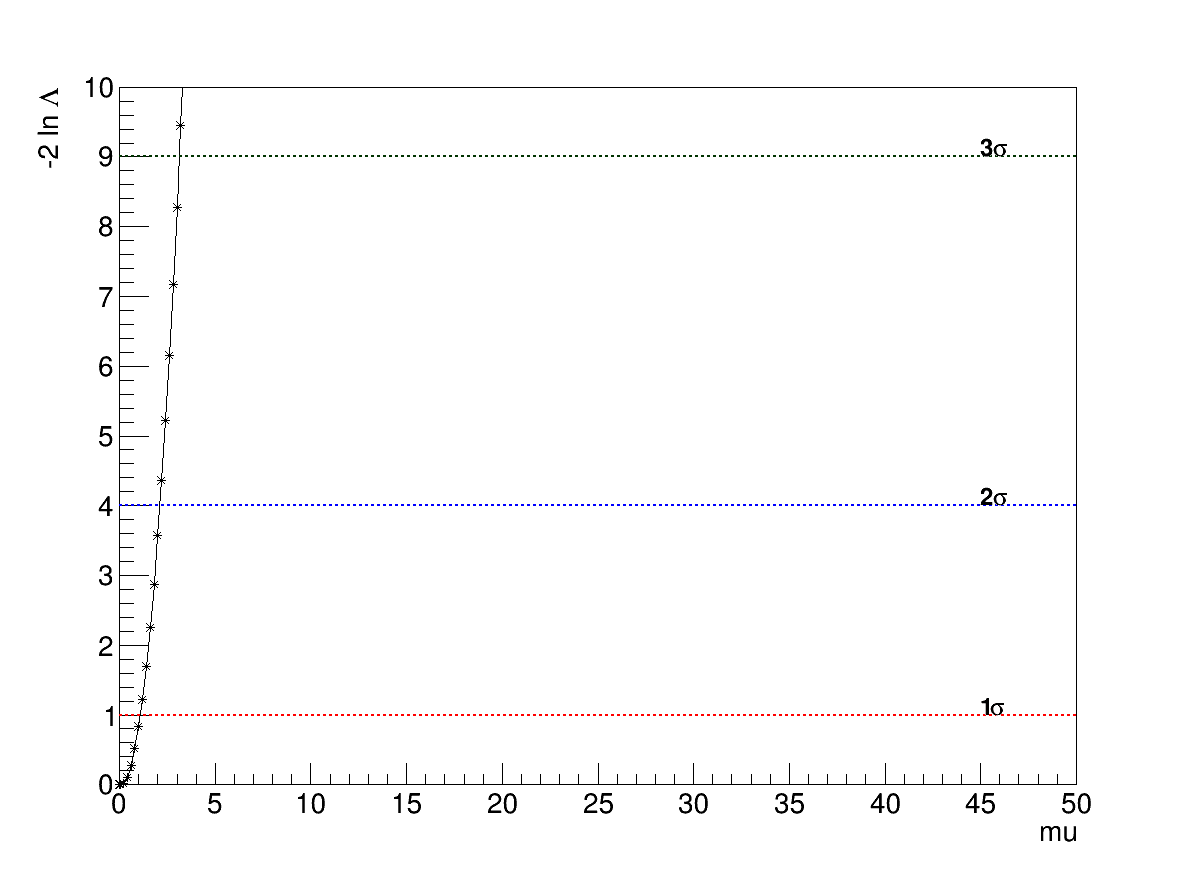
\includegraphics[width=6cm,height=5cm]{figures/Likelihood-kt-1.png}
			\caption*{Likelihood scan for k$_t$=-1}
		\end{figure}
	\end{center}
\end{minipage}
\end{frame}

\begin{frame}
\frametitle{Estimation of $\mu$}
Limit value for $\mu$ for $3\sigma$ 
\begin{tabular}{|c|c|}
kt=1 &  28.047  \\
kt=-1 & 1.97 \\
kt=1 for 150 fb &13.816 \\
kt=1 for 300 fb & 10.491\\
kt=1 for 3000 fb &  4.373 \\
kt=-1 for 150 fb &1.979 \\
kt=-1 for 300 fb &1.713 \\
kt=-1 for 3000fb & 1.181
\end{tabular}
\end{frame}

\begin{frame}
\frametitle{Extrapolation of luminosity }
\begin{center}
\begin{tabular}{cc}
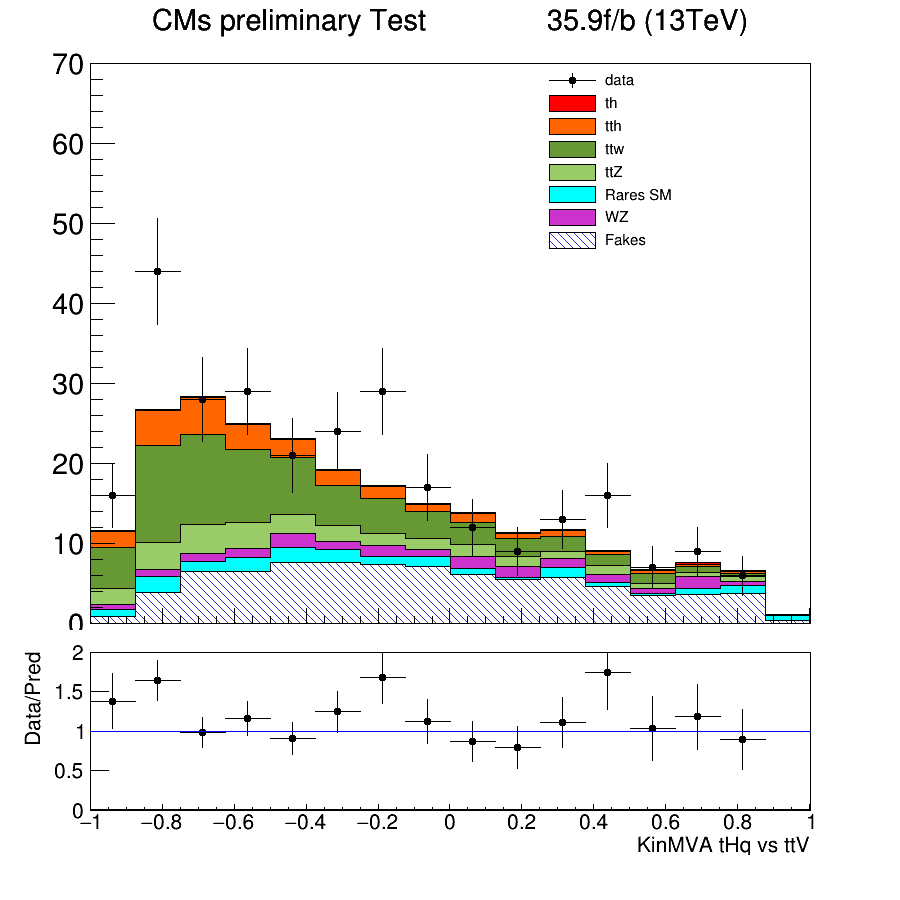
\includegraphics[width=4cm,height=3cm]{figures/kin.png} &
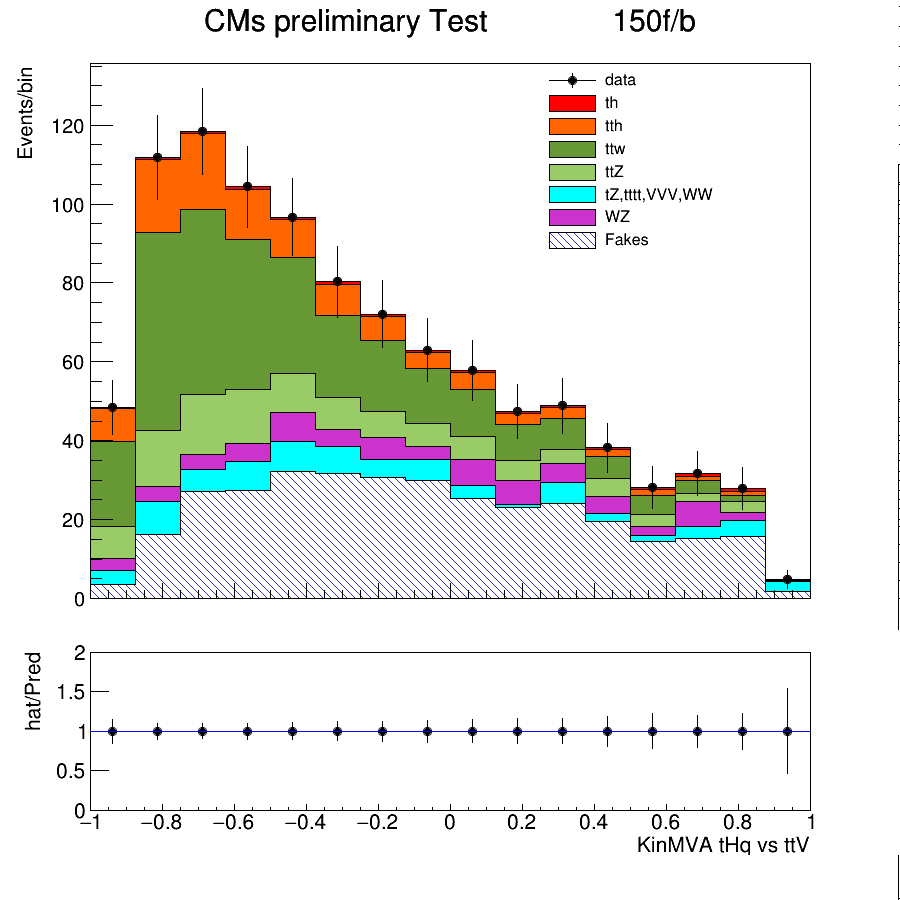
\includegraphics[width=4cm,height=3cm]{figures/150fb/kin.png}\\ 
35.9 fb$^{-1}$ & 150 fb$^{-1}$ \\
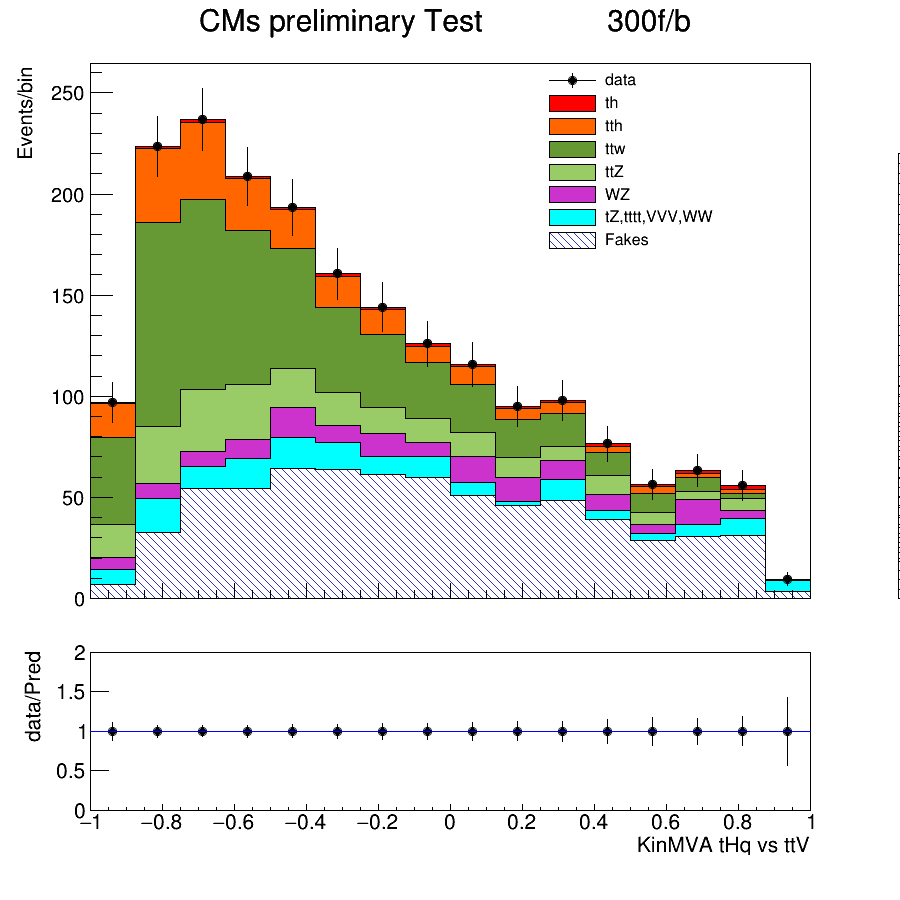
\includegraphics[width=4cm,height=3cm]{figures/300fb/kin-300.png}&
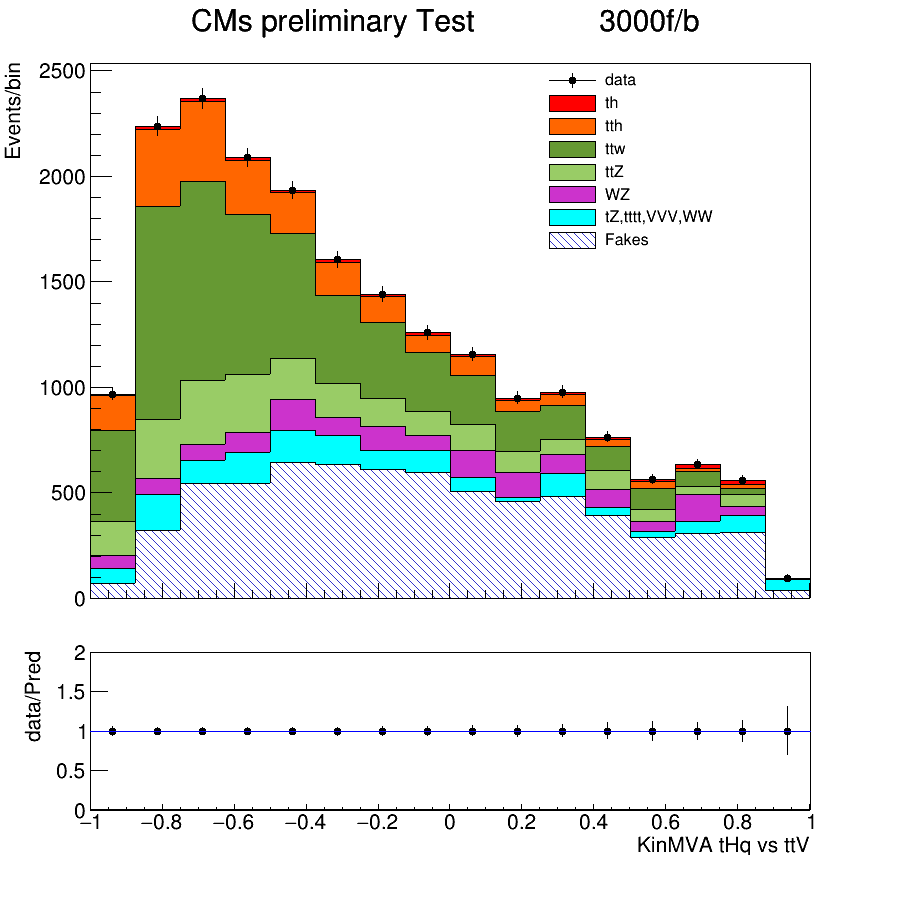
\includegraphics[width=4cm,height=3cm]{figures/3000fb/kin-3000.png}\\
300 fb$^{-1}$ & 3000 fb$^{-1}$ \\
\end{tabular}
\end{center}
\end{frame}


	\begin{thebibliography}{99}
	\begin{frame}
	\section{References}
	\frametitle{References}

	\bibliographystyle{amsalpha}
	\bibitem{1}Gross F. \textit{Relativistic quantum mechanics and field theory} 1994 Wiley
		\bibitem{2}The CMS collaboration, \textit{Search for production of a Higgs boson and a single top
	quark in multilepton final states in proton collisions at 13 TeV}, CMS-PAS-HIG-17-
	005
	\bibitem{3}Verkerke W \textit{Dealing with systematic uncertainties} 2014. From
\url{https://indico.cern.ch/event/287744/contributions/1641261/attachments/535763/738679/Verkerke_Statistics_3.pdf}
\end{frame}

\begin{frame}
\bibitem{5} ATLAS and CMS
Collaborations, \textit{Combined measurement of the Higgs boson mass in
	pp collisions at $\sqrt{s}$= 7 and 8 TeV with the ATLAS and CMS experiments}, Phys. Rev. Lett.
114 (2015) doi:10.1103/PhysRevLett.114.191803, arXiv:1503.07589
\bibitem{4} Cowan G. , Cranmer K., Gross E. , Vitells O.\textit{ Asymptotic formulae for
	likelihood-based tests of new physics} 2013 , arXiv:1007.1727
\bibitem{6} CMS Collaboration, \textit{Search for the tH(H$\rightarrow b \bar{b}$) process in the pp collisions at $
	\sqrt{s}$=13 TeV and study of Higgs boson couplings} 2018,CMS PAS HIG-17-016
\bibitem{7}CMS collaboration \textit{Search for tHq production in multilepton final states at 13 TeV} ,2017,CMS AN-16-378

\end{frame}
\end{thebibliography}

\begin{frame}
\section{Supportive slides}
\huge{Back up}
\end{frame}

\begin{frame}
\frametitle{BDT parameters}

\begin{itemize}
\item Gradient boosted (BDTG)
\item No. of trees = 800
\item No. of cuts = 50
\item Maximum depth = 3
\item Found to be most discriminating, minimal overtraining.
\end{itemize}
\end{frame}

\begin{frame}
\begin{center}
	\begin{figure}
		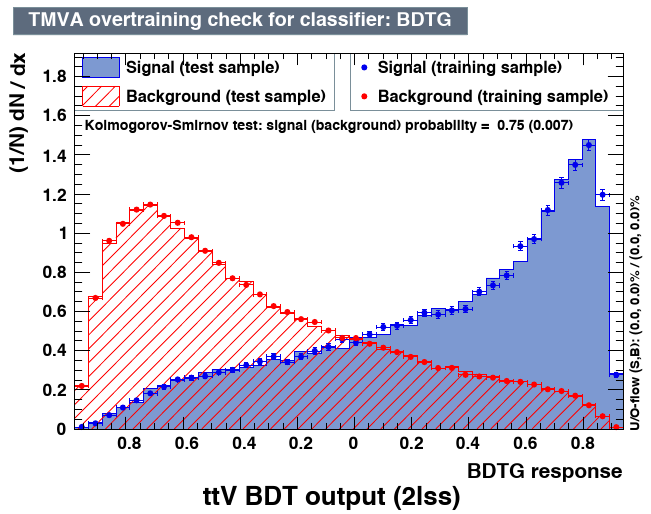
\includegraphics[scale=0.5]{figures/sk.png}
	\end{figure}
\end{center}
\end{frame}

\begin{frame}
\frametitle{List of histograms used in the analysis}
Data taken from the file \texttt{plots-thq-2lss-kinMVA.root} 2016 CERN 
\begin{alltt}
thqMVA\_ttv\_2lss\_40\_tZq \\
thqMVA\_ttv\_2lss\_40\_ttZ\\
thqMVA\_ttv\_2lss\_40\_VVV\\
thqMVA\_ttv\_2lss\_40\_ttW\\
thqMVA\_ttv\_2lss\_40\_data\_fakes\\
thqMVA\_ttv\_2lss\_40\_ttH\\
thqMVA\_ttv\_2lss\_40\_tHW\_hww\\
thqMVA\_ttv\_2lss\_40\_WWss\\
thqMVA\_ttv\_2lss\_40\_tttt\\
thqMVA\_ttv\_2lss\_40\_WZ\\
thqMVA\_ttv\_2lss\_40\_tHq\_hww\\
\end{alltt}
\end{frame}

\begin{frame}
\frametitle{Backgrounds and signal histograms}
\textbf{tHq: Signal (tH)}\\
\begin{itemize}
\item \begin{alltt} thqMVA\_ttv\_2lss\_40\_tHq\_hww \end{alltt}
\item \begin{alltt} thqMVA\_ttv\_2lss\_40\_tHW\_hww \end{alltt}
\end{itemize}
\textbf{Backgrounds} \\
t$\bar{t}$W
\begin{itemize}
\item \begin{alltt} thqMVA\_ttv\_2lss\_40\_ttW\end{alltt}
\end{itemize}
t$\bar{t}$Z
\begin{itemize}
\item \begin{alltt}thqMVA\_ttv\_2lss\_40\_ttZ\end{alltt}
\end{itemize}
WZ
\begin{itemize}
\item \begin{alltt}thqMVA\_ttv\_2lss\_40\_WZ	\end{alltt} 
\end{itemize}


\end{frame}

\begin{frame}
\frametitle{Backgrounds and signal histograms}
\textbf{Backgrounds} \\
tZ, VVV,tttt,WW:
\begin{itemize}
	\item \begin{alltt}thqMVA\_ttv\_2lss\_40\_tZq\end{alltt}
	\item \begin{alltt} thqMVA\_ttv\_2lss\_40\_WWss \end{alltt}
	\item \begin{alltt}thqMVA\_ttv\_2lss\_40\_VVV\end{alltt}
	\item \begin{alltt}thqMVA\_ttv\_2lss\_40\_tttt\end{alltt}
\end{itemize}
t$\bar{t}$H 
\begin{itemize}
	\item\begin{alltt} thqMVA\_ttv\_2lss\_40\_ttH\end{alltt}
\end{itemize}
Non prompt leptons (fakes)
\begin{itemize}
	\item\begin{alltt} thqMVA\_ttv\_2lss\_40\_data\_fakes\end{alltt}
\end{itemize} 
\end{frame}

\begin{frame}

Closure:  hay jets en los eventos de tt  (gluon-gluon -> tt + gluon ) que se pasan como muones.  jet -> muon =  fake

Fakes:   proceso de QCD  que genera muchos  jets (por ejemplo  gluon-gluon -> gluons, quarks)  :    jet -> muons  
fakes are estimated data 


\footnote[1]{Due to existence of many uncertainties, it is neccesary to sum all the uncertainties. When there is no Correlation, the uncertanties must be summed as the square root of the squares of each uncertainty}
\end{frame}


\begin{frame}
\frametitle{Sources of systematic uncertainty}
Detector-simulation related uncertainty
\begin{itemize}
\item Calibrations (electron, jet energy scale)
\item Efficiencies (particle ID, reconstruction)
\item Resolutions (jet energy, muon momentum)
\end{itemize}
Theoretical uncertainties
\begin{itemize}
\item  Factorization/Normalization scale of MC generators
\item Choice of MC generator (ME and/or PS, e.g. Herwig vs Pythia)
\end{itemize}
Monte Carlo Statistical uncertainties
\begin{itemize}\item Statistical uncertainty of simulated samples\cite{2} \end{itemize}
\end{frame}

\begin{frame}
\frametitle{Observed events }
\begin{itemize}
	\item After applying the event pre-selection on the dataset, 280 events are observed in the same-sign $\mu\mu$ channel
	\item The events are then sorted into ten categories depending on the output of the two BDT classifiers
	according to an optimized binning strategy, resulting in a one-dimensional histogram with ten
	bins.
	\item In each point, the tH and t$\bar{t}$H production cross sections and the Higgs decay branching ratios are modified with the Higgs-top ($\kappa_t$) and Higgs-vector boson ($\kappa_v$ ) coupling strength.
	\item  The Higgs-tau coupling strength modifier ($\kappa_\tau$ ) is assumed to be equal to $\kappa_t$ . 
	\item All other parameters are assumed to be at the values predicted by the standard model\cite{1}	.
\end{itemize}
\end{frame}


\begin{frame}
\frametitle{$\alpha$ values for post fit}
\begin{alltt}
Floating Parameter		\qquad		FinalValue +/- Error \\
$-----------------------------------------------------------------------$			
Lumi \quad	\qquad	\qquad		\qquad	\qquad	1.0082e+00 +/-  2.42e-02\\
alpha\_sample\_tth\_sys	\quad	1.9100e-01 +/-  9.94e-01\\
alpha\_sample\_ttw\_sys	\quad	8.7537e-01 +/-  9.18e-01\\
alpha\_sample\_ttz\_sys	\quad	2.0012e-01 +/-  9.95e-01\\
alpha\_sample\_tz\_sys\qquad	1.6749e-01 +/-  1.00e+00\\
alpha\_sample\_wz\_sys\qquad	 1.2732e-01 +/-  9.84e-01 \\
alpha\_sample\_fakes\_sys	4.5030e-01 +/-  7.17e-01\\
mu 	\qquad	\qquad	\qquad	\qquad	\qquad	2.4975e+00 +/-  1.29e+01
\end{alltt}
\end{frame}

\begin{frame}
\frametitle{$\alpha$ values for post fit thq $k_t$=-1}
\begin{alltt}
Floating Parameter			\qquad		FinalValue +/- Error \\
$-----------------------------$
Lumi \quad	\qquad	\qquad		\qquad	\qquad 1.0085e+00 +/-  2.40e-02\\
alpha\_sample\_tth\_sys	\quad	1.9290e-01 +/-  1.00e+00 \\
alpha\_sample\_ttw\_sys	\quad	8.7911e-01 +/-  9.42e-01\\
alpha\_sample\_ttz\_sys	\quad	2.0370e-01 +/-  9.94e-01\\
alpha\_sample\_tz\_sys\qquad	1.8269e-01 +/-  9.69e-01\\
alpha\_sample\_wz\_sys\qquad	1.4244e-01 +/-  9.99e-01\\
alpha\_sample\_fakes\_sys	1.4243e-01 +/-  9.98e-01\\
mu \qquad	\qquad	\qquad	\qquad	\qquad 6.9361e-02 +/-  1.02e+00
\end{alltt}
\end{frame}

\begin{frame}
\frametitle{Results}
\framesubtitle{Likelihood scan}
\begin{itemize}
	\item Likelihood function (often simply the likelihood) is a function of the
	parameters of a statistical model, given specific observed data.
	\item Likelihood functions play a key role in frequentist inference,
	especially methods of estimating a parameter from a set of
	statistics.
	\item In informal contexts, "likelihood" is often used as a synonym for
	probability.
\end{itemize}
\end{frame}

\begin{frame}
\frametitle{Statistical test}
It is convenient to use the statistic
\begin{align}
t_\mu=-2\ln{\lambda(\mu)} 
\end{align}
as the basis of a statistical test. Higher values of $t_\mu$ thus correspond to increasing
incompatbility between the data and $\mu$.
We may define a test of a hypothesized value of $\mu$ by using the statistic $t_\mu$ directly
as measure of discrepancy between the data and the hypothesis, with higher values of
$t_\mu$ correspond to increasing disagreement\cite{4}
\end{frame}

\begin{frame}
\frametitle{Statistical test}
\begin{center}
	\begin{figure}
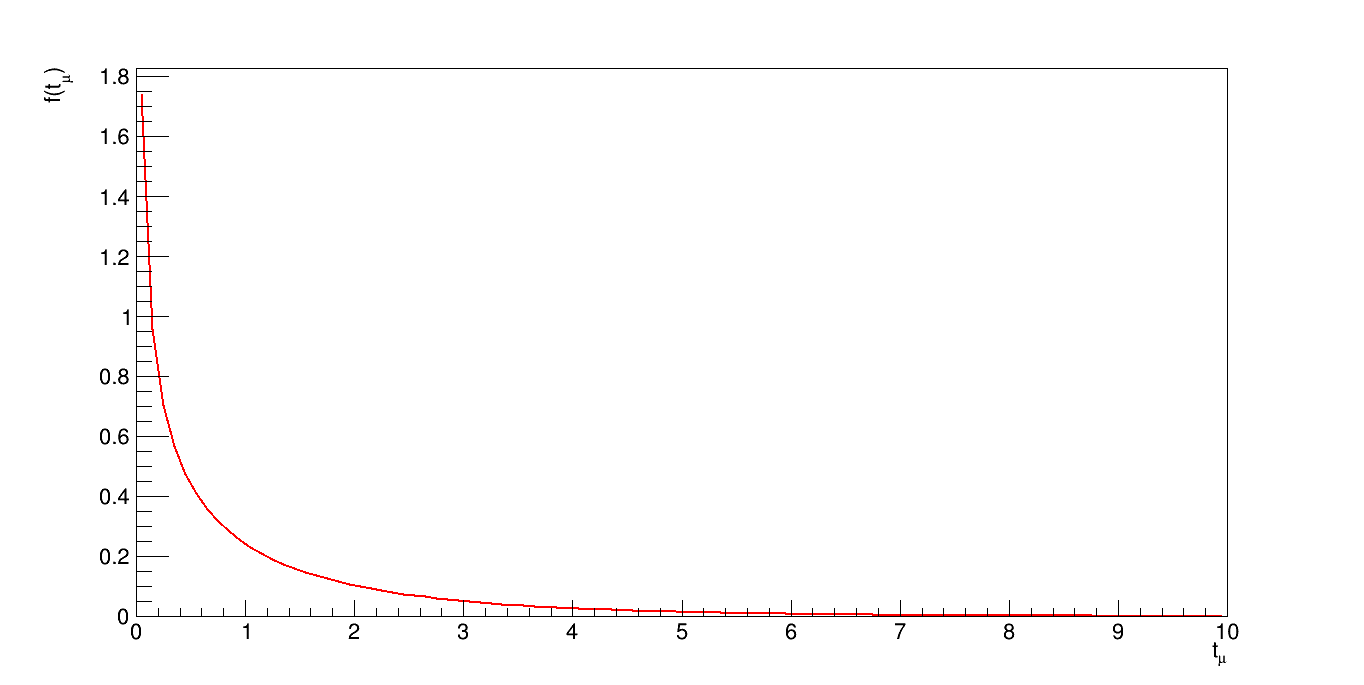
\includegraphics[scale=0.25]{figures/tmu.png}
\caption{Statistic test plot $f(t_\mu)$ vs $t_\mu$ with $t_\mu=-2\ln{\lambda(\mu)}$}
\end{figure}
\end{center}
\end{frame}

\begin{frame}
\frametitle{P value}
To quantify the level of disagreement we compute the P-value
\begin{align}
P_\mu =\int_{t_\mu}^{\infty}f(t\mu |\mu) dt_\mu
\end{align}
where t $\mu$  is the value of the statistic t$\mu$ observed from the data and $f(t\mu |\mu)$ denotes
the PDF (Probability density function) of t$\	mu$ under the assumption of the signal strength $\mu$\cite{4}
\end{frame}

\begin{frame}
\frametitle{P value}
\begin{center}
\begin{figure}
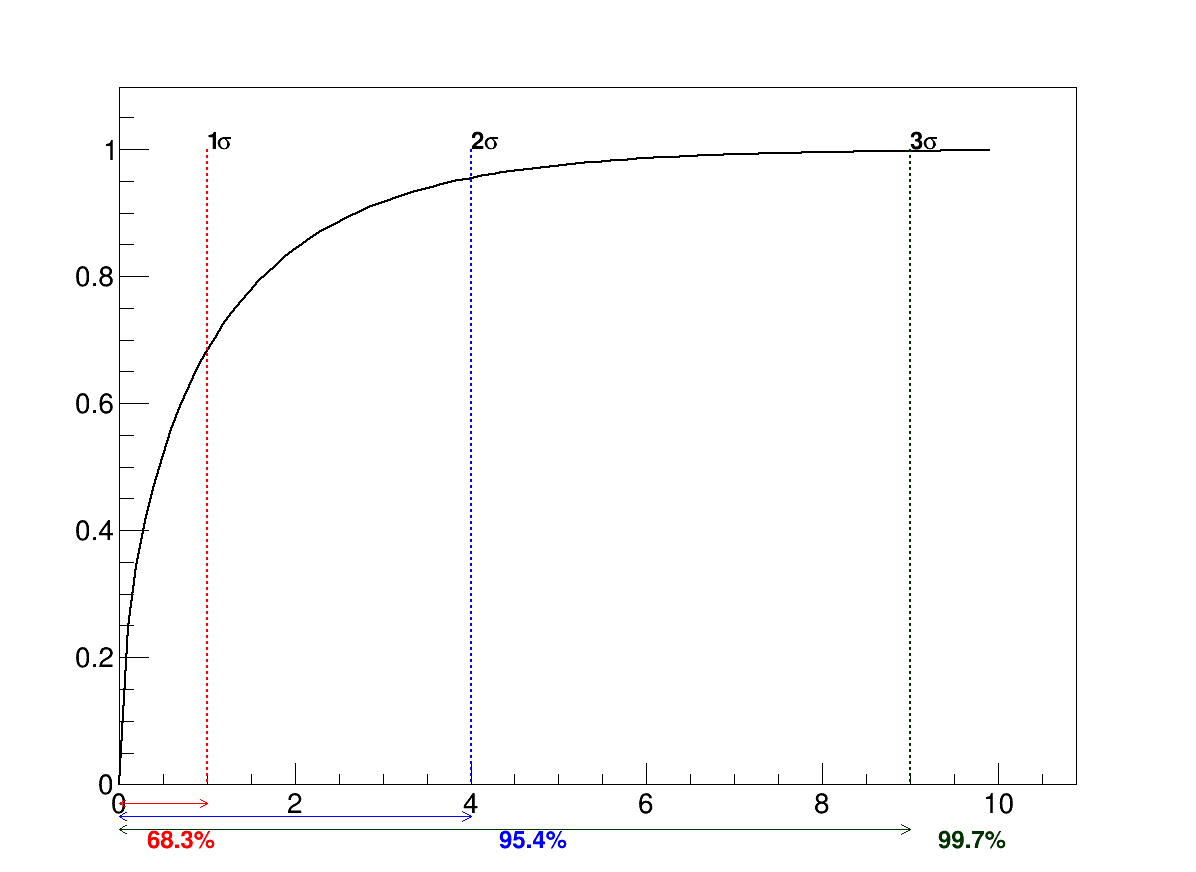
\includegraphics[scale=0.25]{figures/nos.png}
\caption{$P_\mu$ vs  f($t_\mu$|$\mu$)}	
\end{figure}
\end{center}
\end{frame}

\begin{frame}
\frametitle{Luminosity scale}
\framesubtitle{150 fb}
\begin{multicols}{2}
\begin{center}
	\begin{figure}
		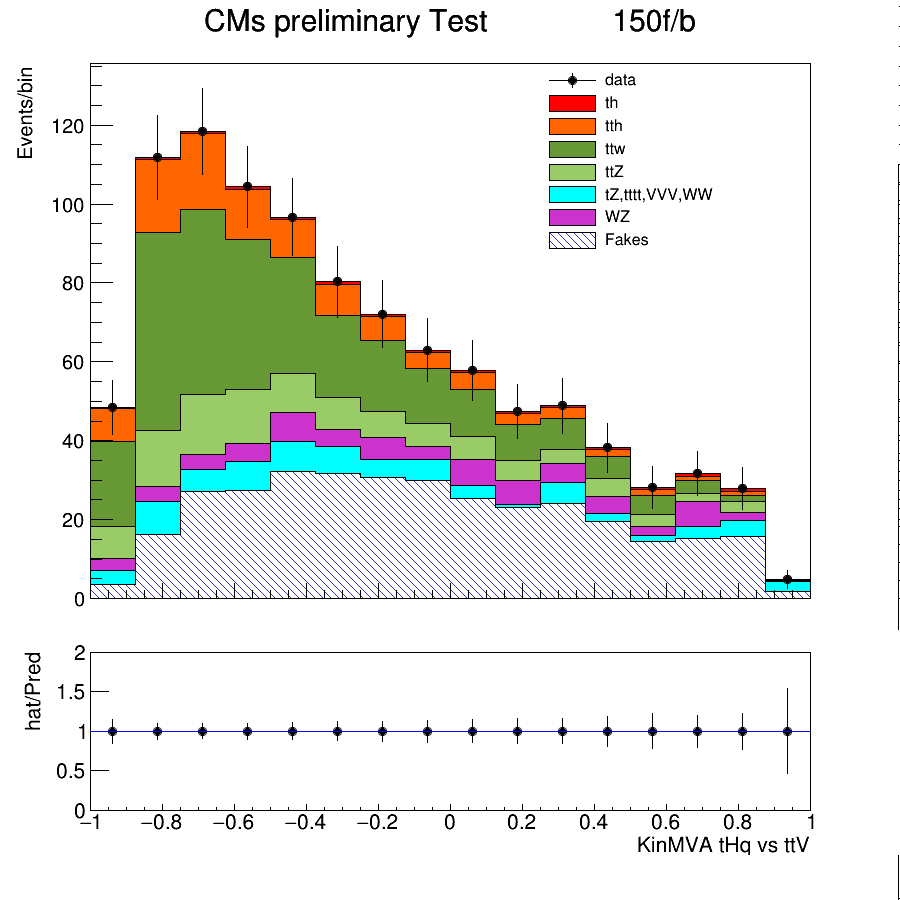
\includegraphics[width=6cm,height=6cm]{figures/150fb/kin.png}
		\caption*{Prefit }
	\end{figure}
\end{center}
\columnbreak
\begin{center}
	\begin{figure}
		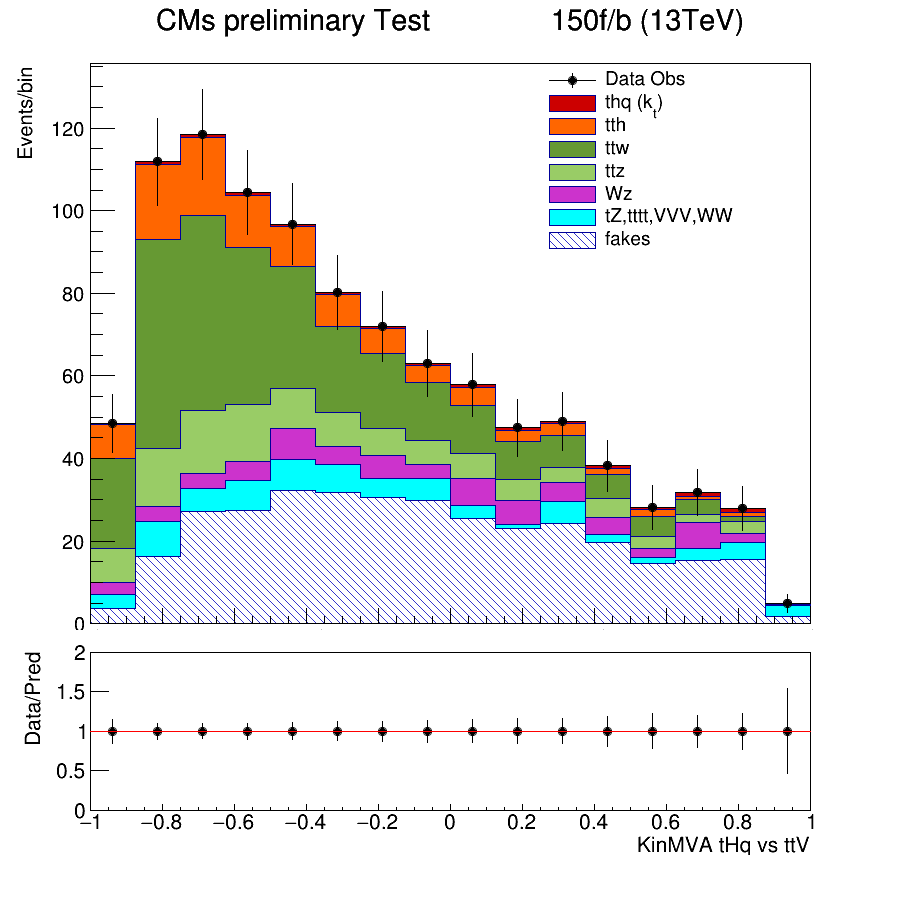
\includegraphics[width=6cm,height=6cm]{figures/150fb/simple.png}
		\caption*{Post fit }
	\end{figure}
\end{center}
\end{multicols}
\end{frame}

\begin{frame}
\frametitle{Luminosity scale}
\framesubtitle{150 fb}
\begin{table}
	\begin{tabular}{|c|c|c|}
		\hline
event  & N prefit    & N Postfit \\
\hline
tH & 8.89972 $\pm$  0.885511 & 8.89972$\pm$57.2784\\
\hline
ttH  & 101.031 $\pm$  9.45& 101.031$\pm$9.27757\\
\hline
ttW  & 284.248$\pm$39.8961  & 284.248$\pm$31.3604\\
\hline
ttZ  & 108.175$\pm$  13.3806 & 108.175$\pm$13.1161\\
\hline
tZ & 71.7409$\pm$34.1567  & 71.7409$\pm$31.8423\\
\hline
WZ & 67.8134 $\pm$ & 67.8134$\pm$31.8861\\
\hline
fakes  & 338.189$\pm$  170.744  & 338.189$\pm$84.302\\
\hline
	\end{tabular}
\end{table}
\end{frame}


\begin{frame}
\frametitle{Luminosity scale}
\framesubtitle{Likelihood scan}
\begin{center}
	\begin{figure}
	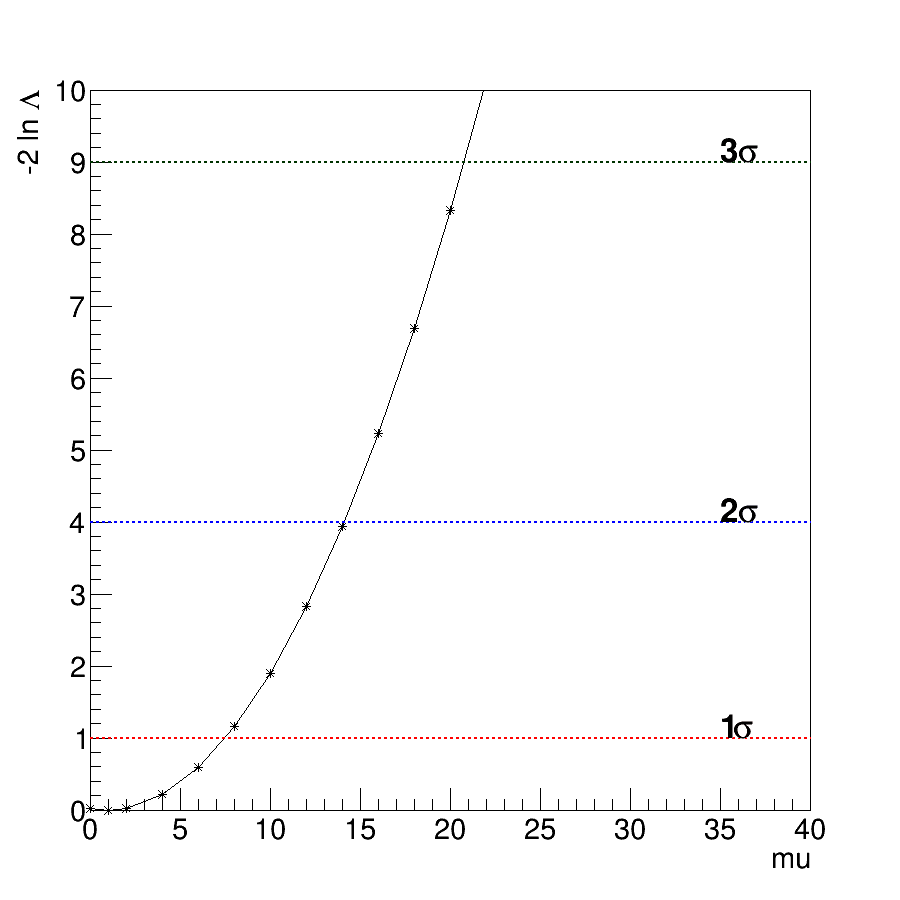
\includegraphics[scale=0.25]{figures/150fb/Likelihood.png}
\end{figure}
\end{center}
\end{frame}

\begin{frame}
\frametitle{Luminosity scale}
\framesubtitle{300 fb}
\begin{multicols}{2}
	\begin{center}
		\begin{figure}
			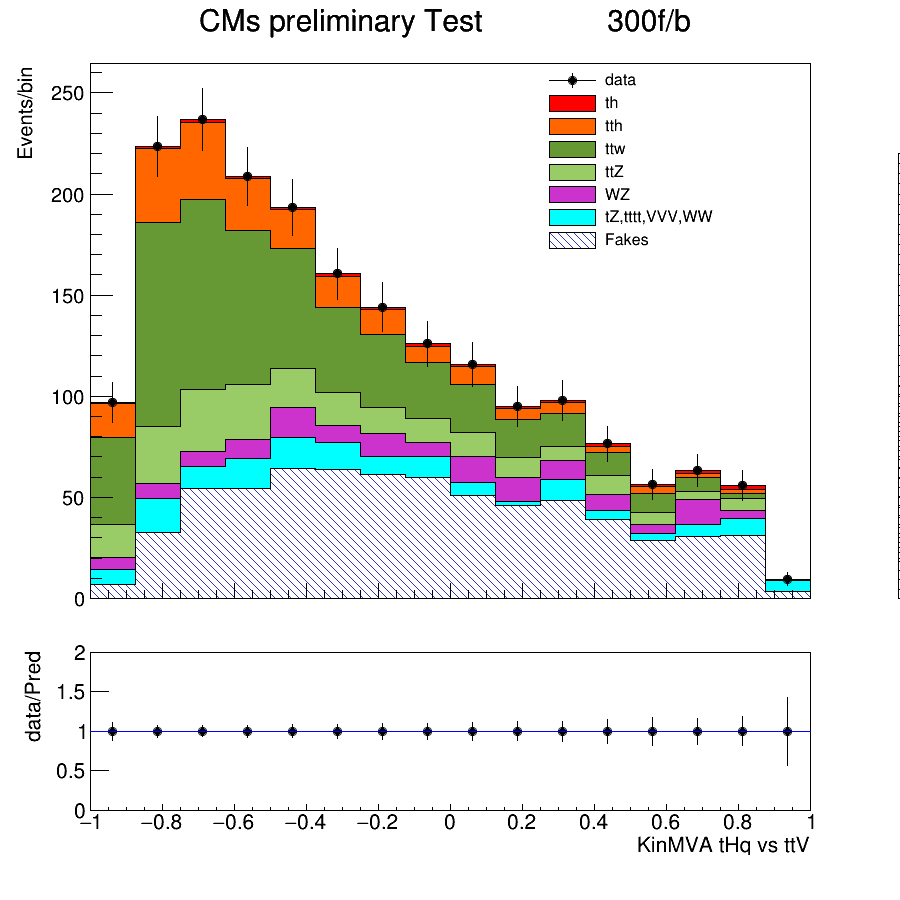
\includegraphics[width=6cm,height=6cm]{figures/300fb/kin-300.png}
				\caption*{Prefit }
		\end{figure}
	\end{center}
	\columnbreak
	\begin{center}
		\begin{figure}
			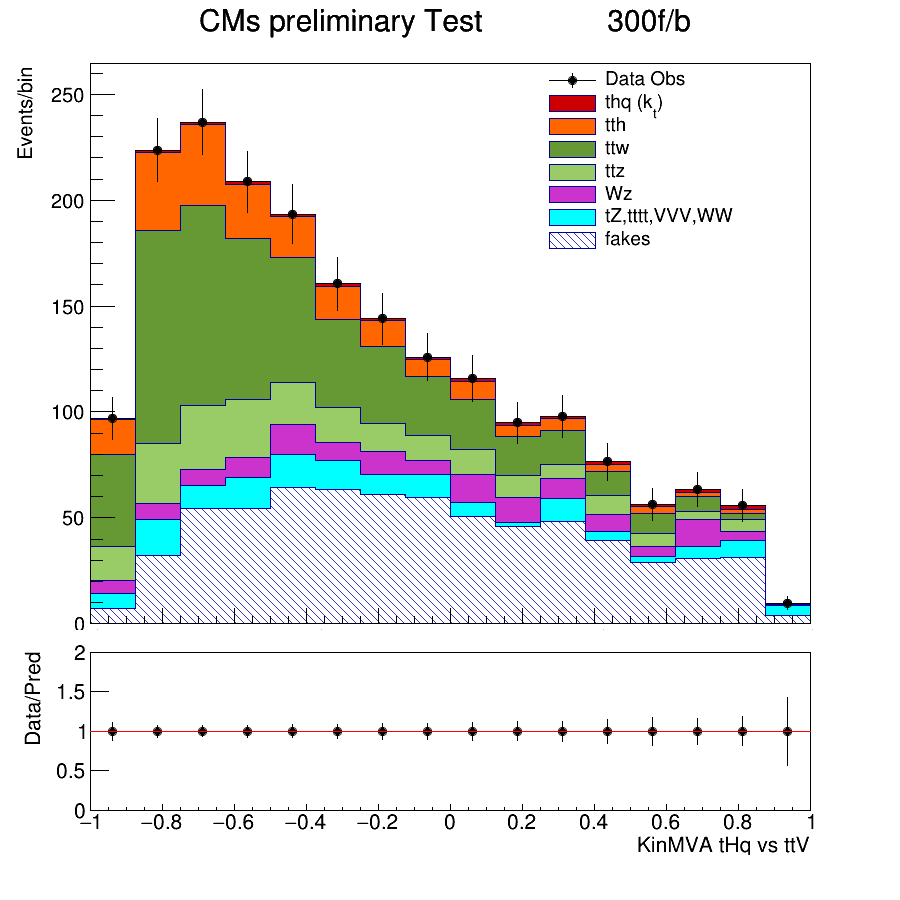
\includegraphics[width=6cm,height=6cm]{figures/300fb/simple.png}
				\caption*{post fit }
		\end{figure}
	\end{center}
\end{multicols}
\end{frame}

\begin{frame}
\frametitle{Luminosity scale}
\framesubtitle{300 fb}
Table of yields for background and signal
\begin{table}
	\begin{tabular}{|c|c|c|}
			\hline
tH & 17.7994 $\pm$ & 17.7994$\pm$85.9204\\
\hline
ttH  & 202.061$\pm$ 18.9162 & 202.061$\pm$18.4728\\
\hline
ttW  & 568.496$\pm$79.7922 & 568.496$\pm$56.3133\\
\hline
ttZ  & 216.351$\pm$ 26.7611 & 216.351$\pm$26.099\\
\hline
tZ & 143.482$\pm$72.2699 & 143.482$\pm$58.5044\\
\hline
WZ & 135.627 $\pm$68.3133& 135.627$\pm$60.7892\\
\hline
fakes  & 676.379$\pm$ 341.488 & 676.379$\pm$133.725\\
	\hline
	\end{tabular}
\end{table}
\end{frame}


\begin{frame}
\frametitle{Luminosity scale}
\framesubtitle{Likelihood scan}
\begin{center}
	\begin{figure}
		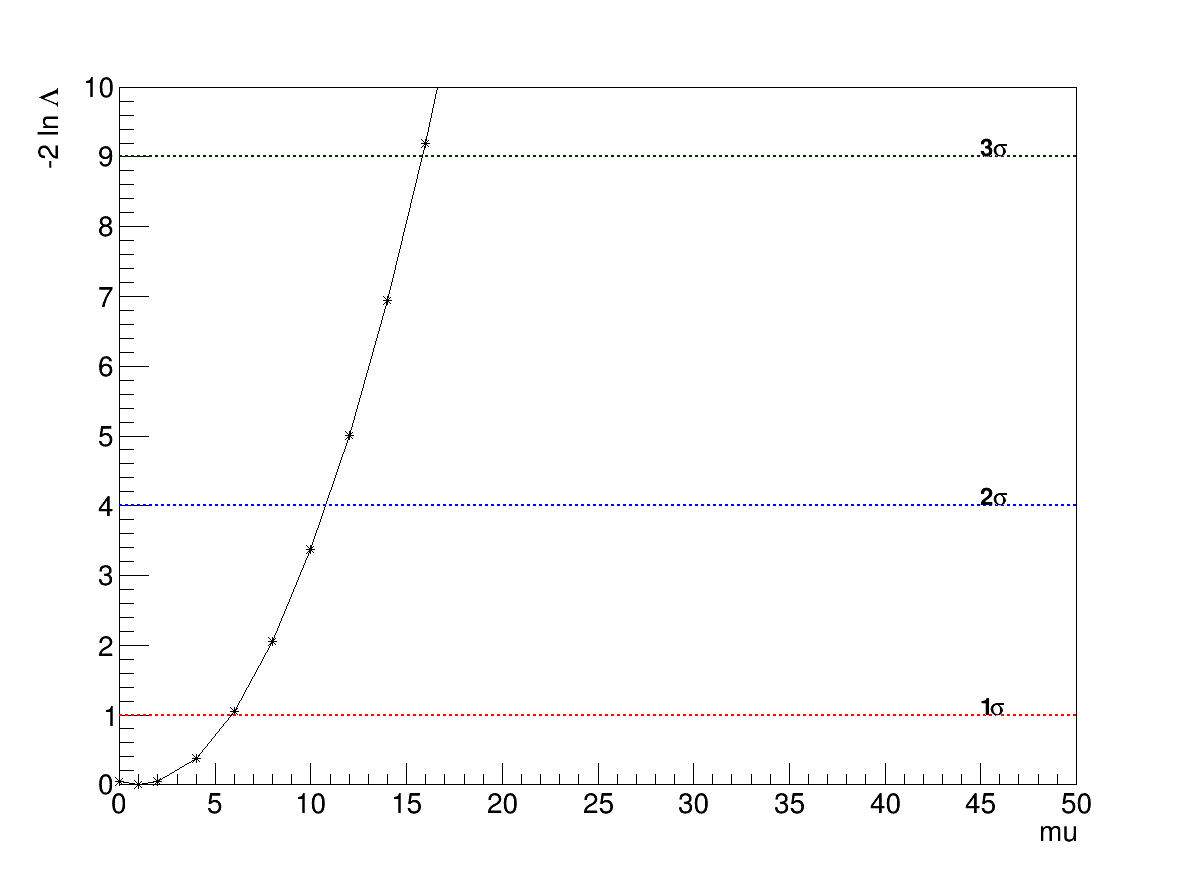
\includegraphics[scale=0.25]{figures/300fb/Likelihood.png}
	\end{figure}
\end{center}
\end{frame}




\begin{frame}
\frametitle{Luminosity scale}
\framesubtitle{3000 fb}
\begin{multicols}{2}
	\begin{center}
		\begin{figure}
			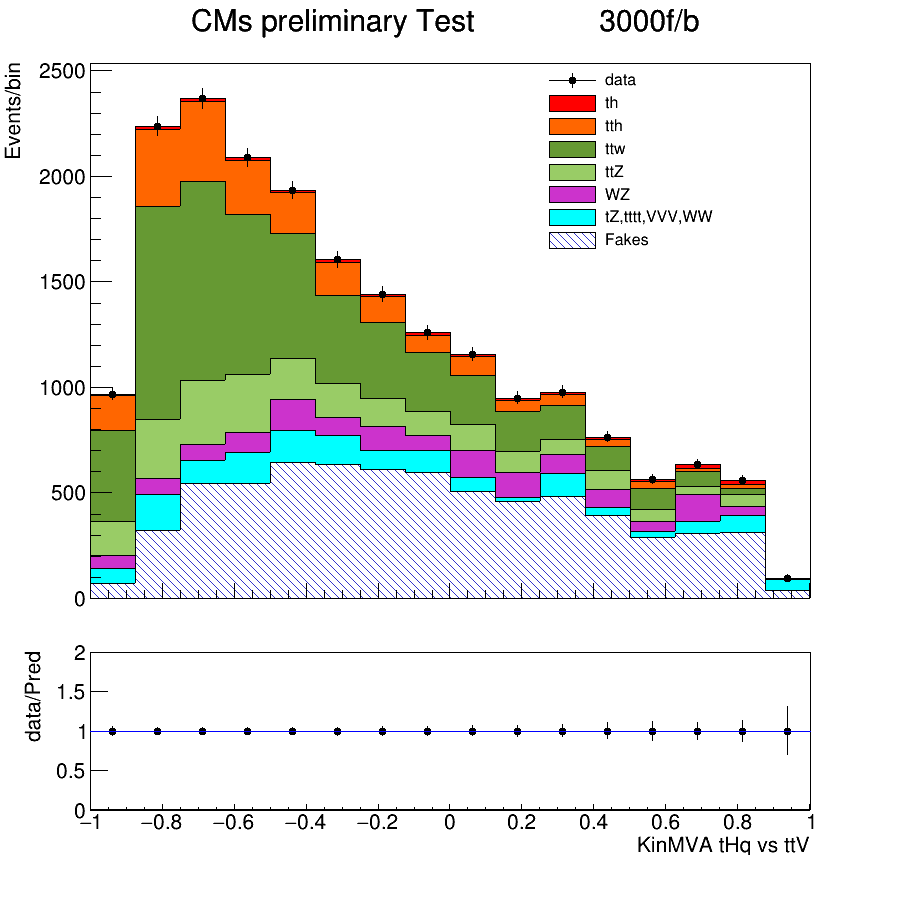
\includegraphics[width=6cm,height=6cm]{figures/3000fb/kin-3000.png}
				\caption*{Prefit }
		\end{figure}
	\end{center}
	\columnbreak
	\begin{center}
		\begin{figure}
			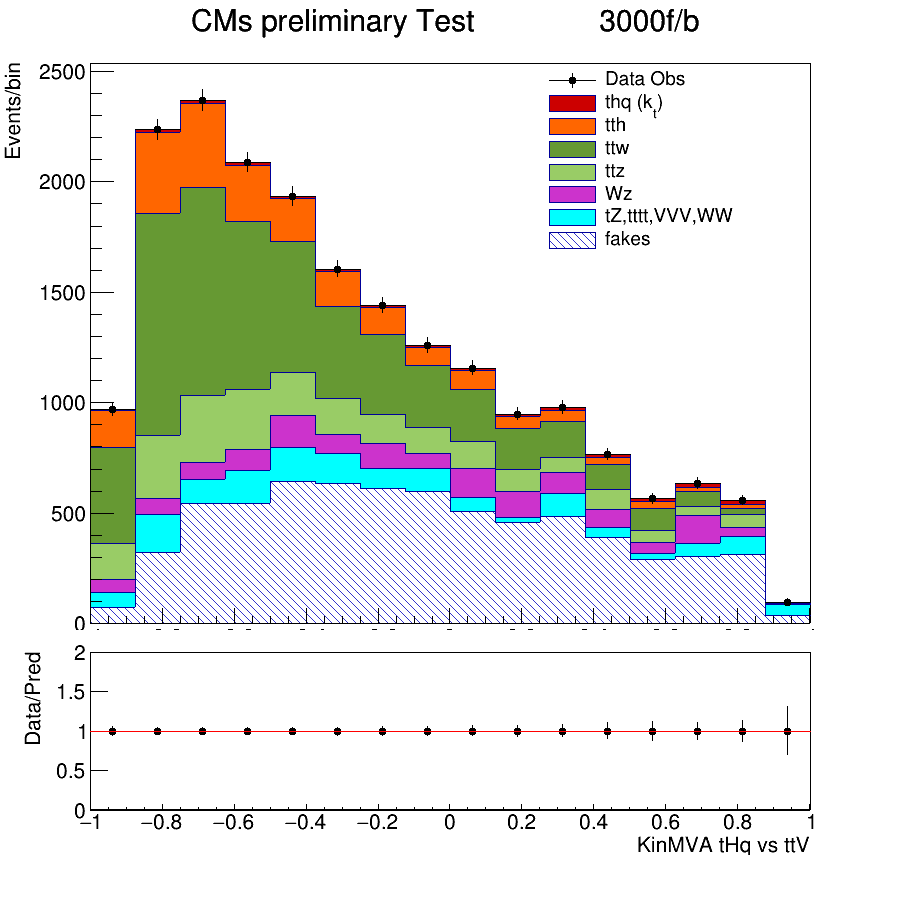
\includegraphics[width=6cm,height=6cm]{figures/3000fb/simple.png}
				\caption*{Post fit }
		\end{figure}
	\end{center}
\end{multicols}
\end{frame}

\begin{frame}
\frametitle{Luminosity scale}
\framesubtitle{3000 fb}
Table of yields for background and signal
\begin{table}
	\begin{tabular}{|c|c|c|}
		\hline
event  & N prefit    & N Postfit \\
\hline
tH & 5076.72 $\pm$505.128 & 5076.72$\pm$643.706\\
\hline
ttH  & 2020.61$\pm$189.162 & 2020.61$\pm$183.997\\
\hline
ttW  & 5684.96$\pm$  797.922& 5684.96$\pm$561.487\\
\hline
ttZ  & 2163.51$\pm$267.611 & 2163.51$\pm$256.289\\
\hline
tZ & 1434.82$\pm$722.699 & 1434.82$\pm$303.361\\
\hline
WZ & 1356.27$\pm$ 683.133& 1356.27$\pm$383.271\\
\hline
fakes  & 6763.79 $\pm$3414.88 & 6763.79$\pm$591.597\\
	\hline
	\end{tabular}
\end{table}
\end{frame}

\begin{frame}
\frametitle{Luminosity scale}
\framesubtitle{Likelihood scan}
\begin{center}
	\begin{figure}
		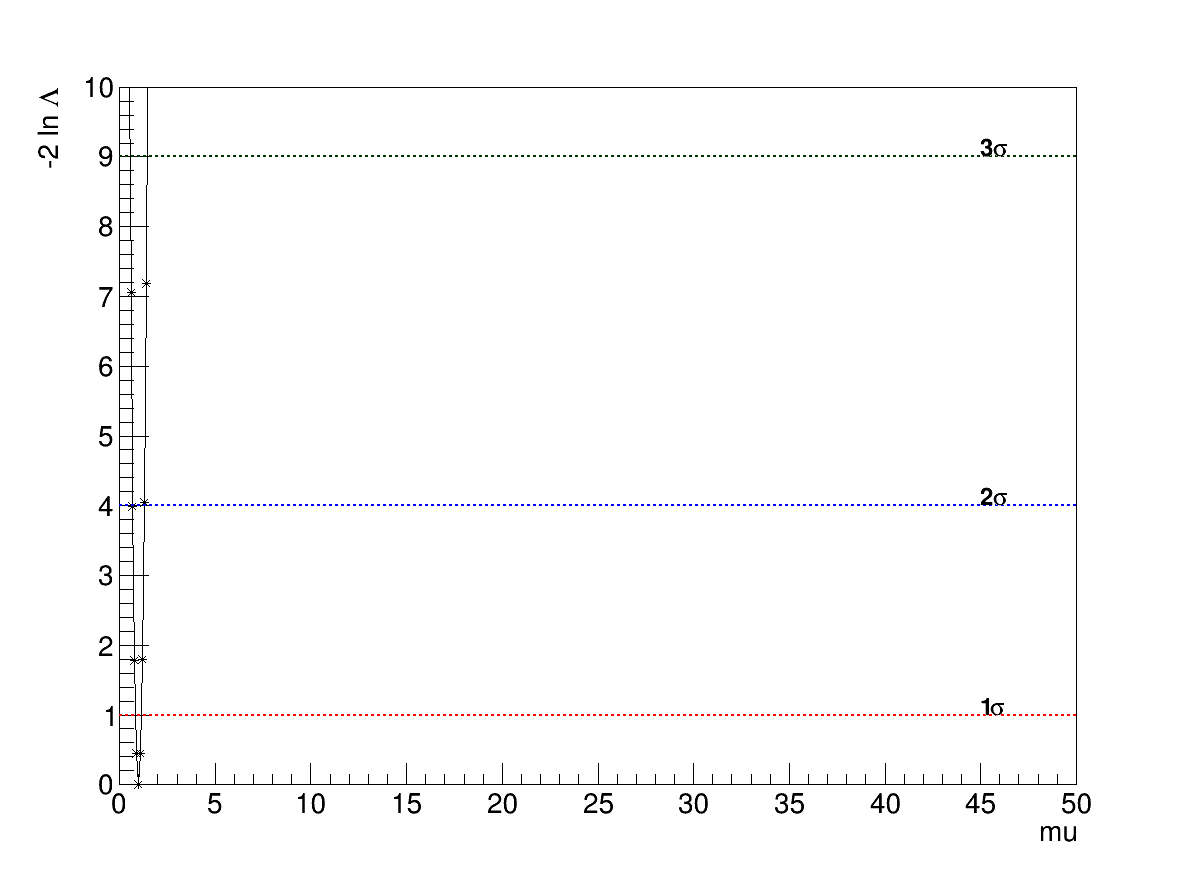
\includegraphics[scale=0.25]{figures/3000fb/Likelihood.png}
	\end{figure}
\end{center}
\end{frame}




\end{document}